\chapter{Validation of the simulation}
\label{appendix:SimulationVal}

\section{Beam profiles}

The simulation needs as one input the position and width of the particle gun. It has to be placed in x, y directions such that the beam sizes of the experiment are modeled and in order to garanty that the same cells of the detector are hit in the simulation as in data. Otherwise, dead and noisy channels could bias the comparison between data and simulation. In the z direction, the beam gun needs to be put as close as possible of the detector to avoid beam broadening by scatering on air molecules.

The best method to estimate the beam profile for data would be to analyse the beam profile provided by the wired chambers. Unfortunately, this data is not available for this analysis. As a work-around, the mean and RMS of the center of gravity distributions in x and y are used to estimate the beam size instead. This does not reflect the true positions since both positions are biased by dead and noisy channels. This has been done for electrons runs as well as for pions runs for each energies. No significant differences in beam profile is visible on a run-by-run basis. The muon beam is simulated by a plane square distribution with a half width of 20 cm. The center of gravity is calculated as the following:

\begin{equation}
  CoG_x [mm] = \frac{\Sigma_i E_i x_i}{\Sigma_i E_i} \quad \text{,} \quad CoG_y [mm] = \frac{\Sigma_i E_i y_i}{\Sigma_i E_i} \quad \text{and} \quad CoG_z [mm] = \frac{\Sigma_i E_i z_i}{\Sigma_i E_i}
\end{equation}

\noindent with $E_i$ the energy of the i-th hit and $x_i$ and $y_i$ the x and y position of the i-th hit.

The beam profiles in the x and y directions for muons is shown in figures \ref{fig:BPmu} for data and simulation. The beam profile is not perfectly reproduced but is good enough. This will have a slight impact on the data and simulation comparison as we are very sensitive to the
profile of the beam.

\begin{figure}[htbp!]
  \centering
  \begin{subfigure}[t]{0.49\textwidth}
    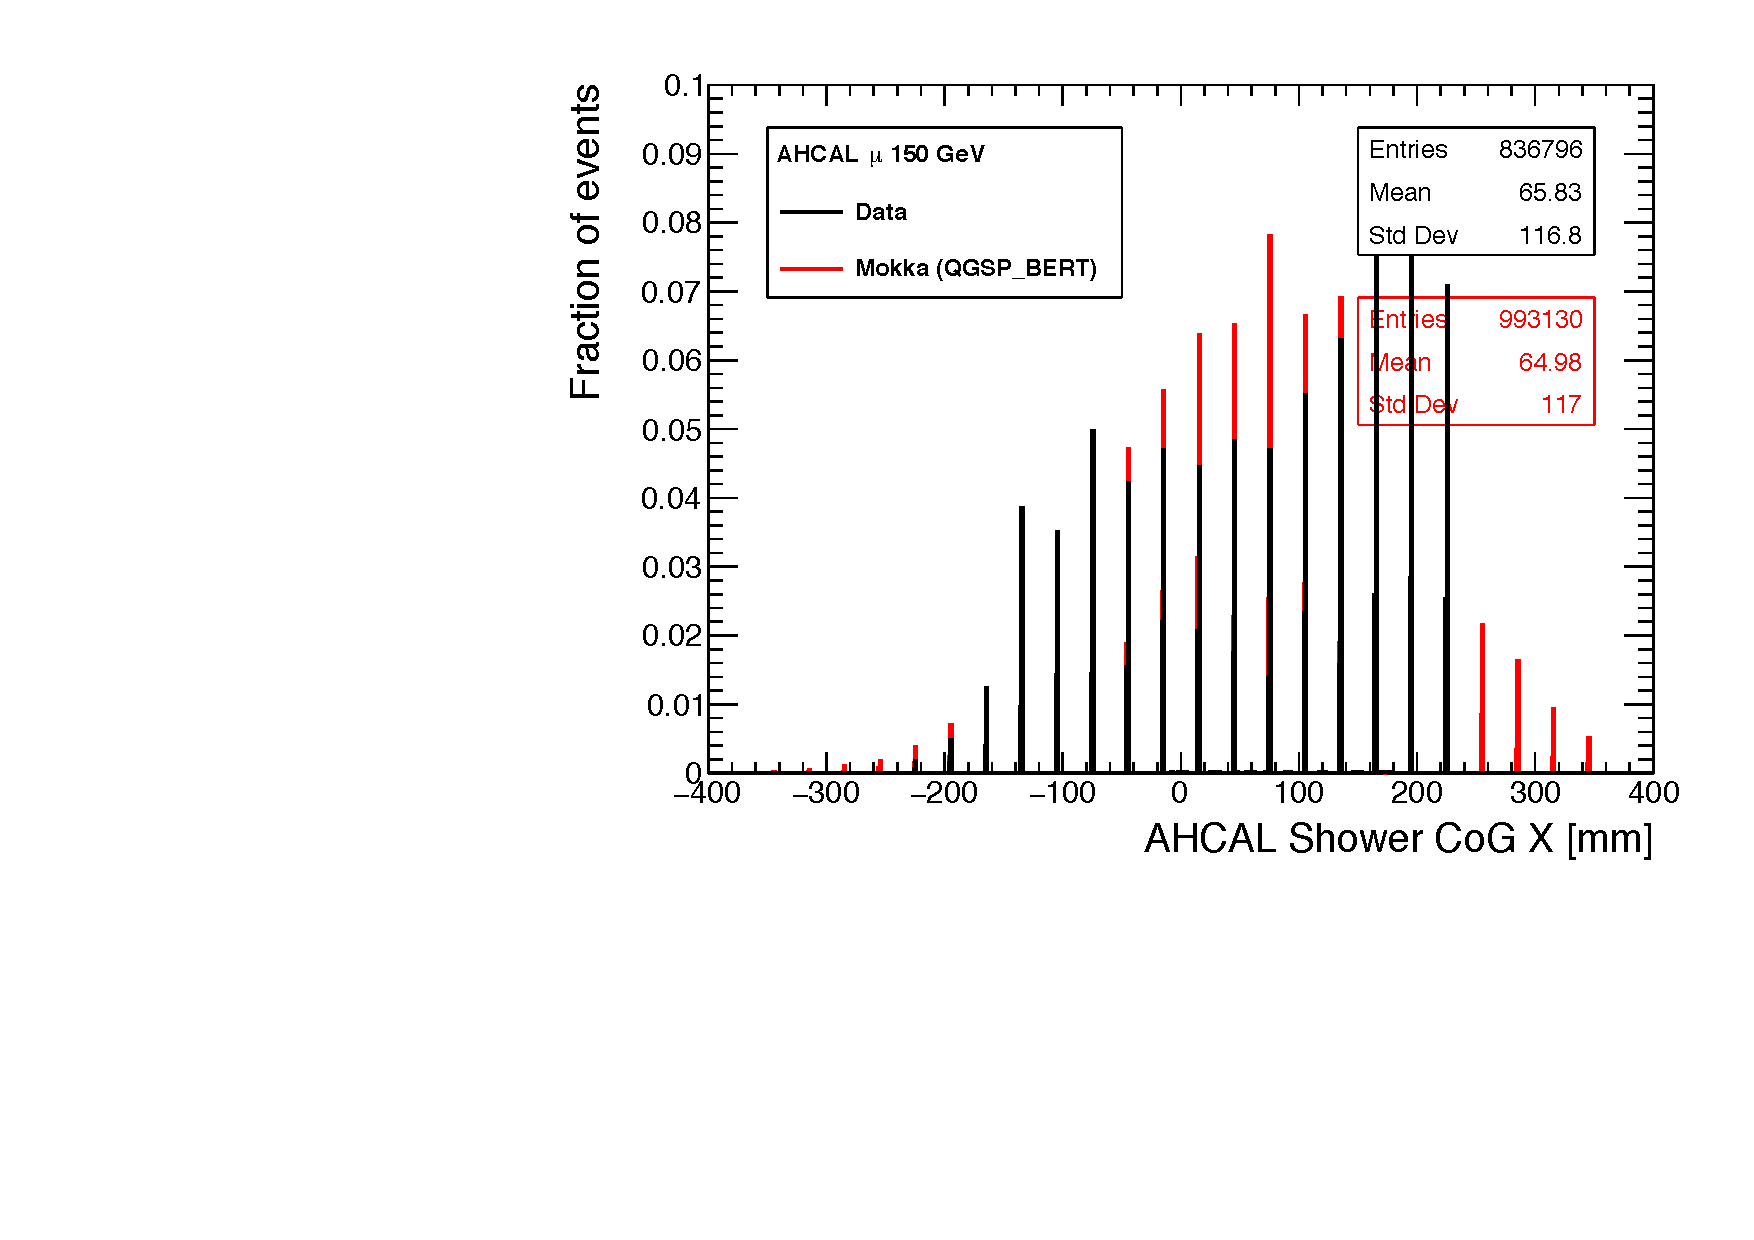
\includegraphics[width=1.\linewidth]{chap5/fig_AHCAL_Timing/Muons/BeamProfileX.pdf}
    \caption{CoG X.} \label{fig:mu150GeVX}
  \end{subfigure}
  \hfill
  \begin{subfigure}[t]{0.49\textwidth}
    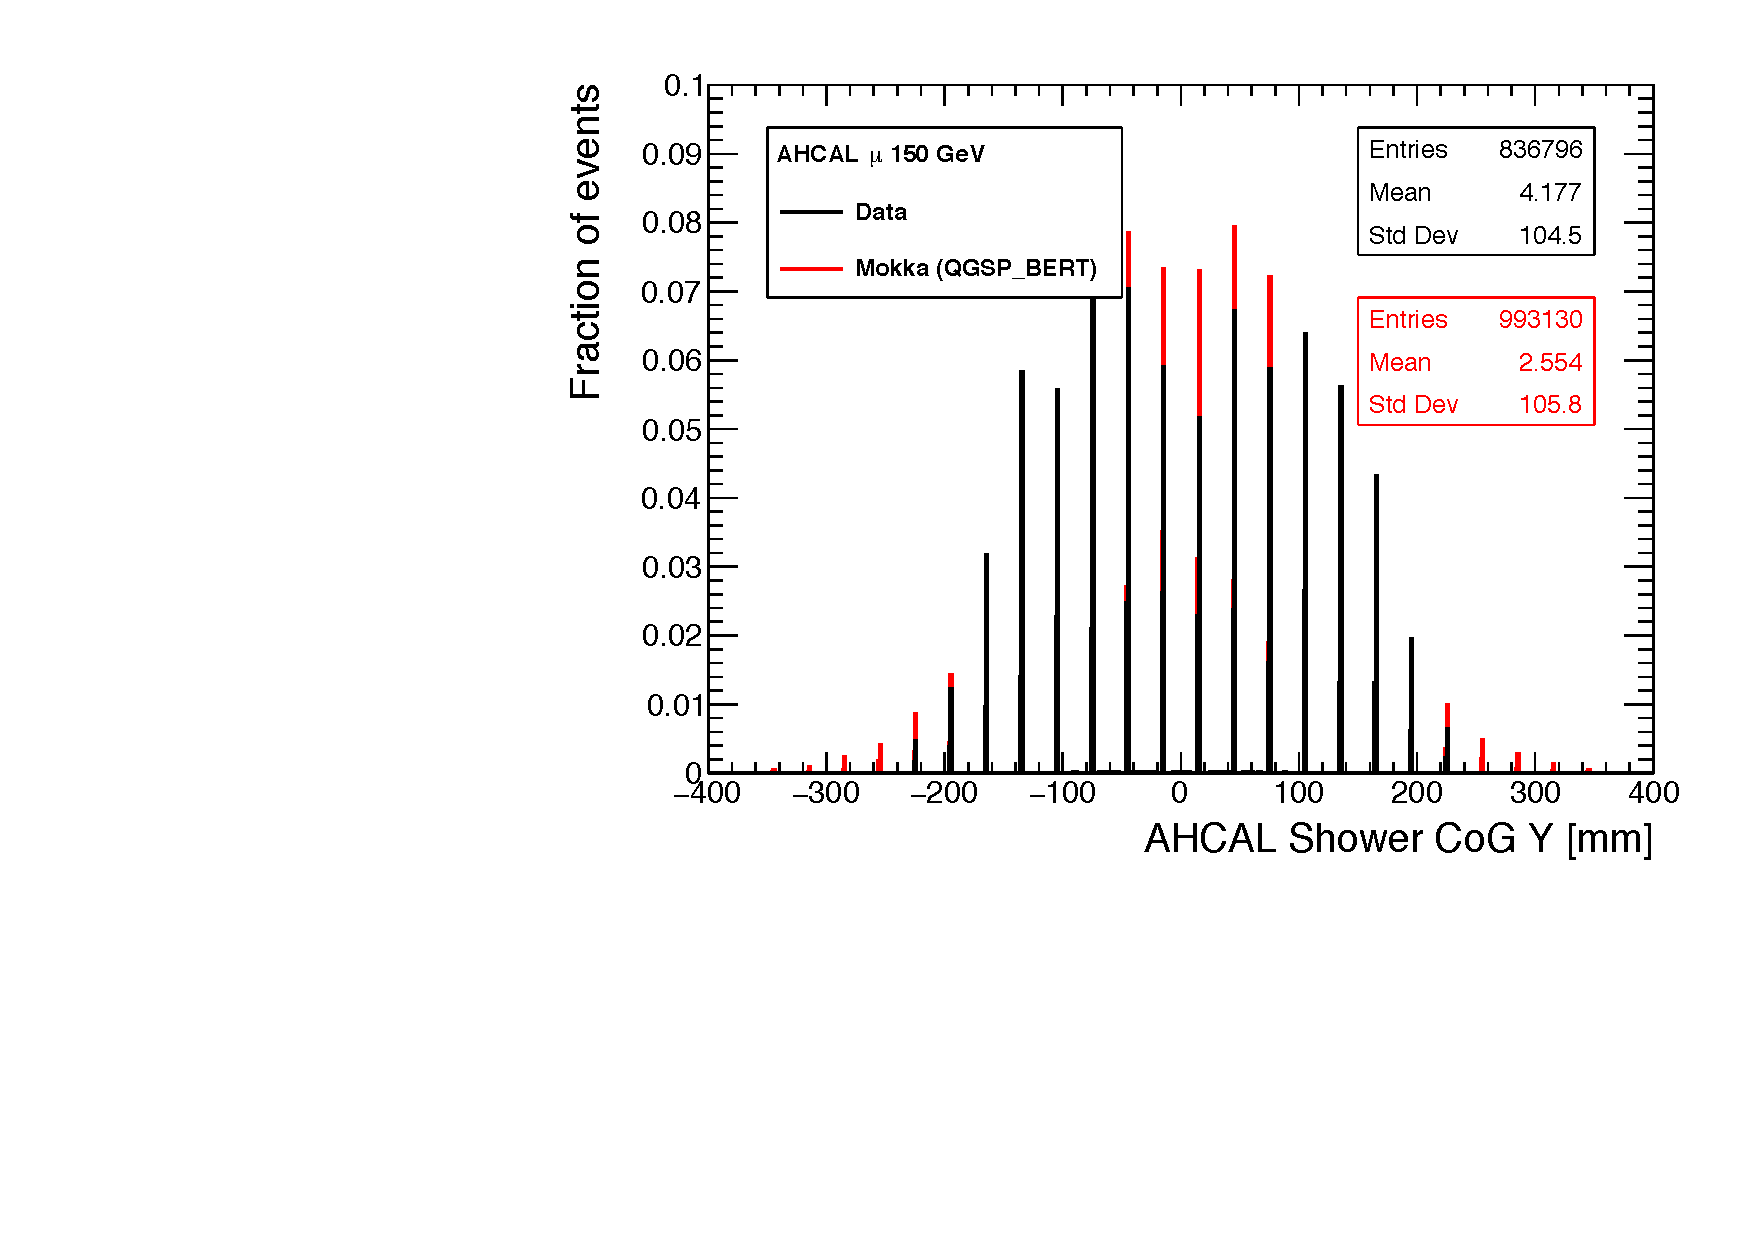
\includegraphics[width=1.\linewidth]{chap5/fig_AHCAL_Timing/Muons/BeamProfileY.pdf}
    \caption{CoG Y.} \label{fig:mu150GeVY}
  \end{subfigure}
  \caption{Beam profiles for 150 GeV muons for data and simulation in the x and y directions.}
  \label{fig:BPmu}
\end{figure}

Figures \ref{fig:BPe} show the beam profiles in the x and y directions for data and simulation for 10 GeV and 50 GeV electrons. The aggrement look much better for 10 GeV than for 50 GeV, this may be due to contamination from lower energy electrons. Moreover, at higher energy, the beam looks less gaussian-like and the shape in simulation can't be simulated correctly. Figures \ref{fig:BPpi} show the beam profiles in the x and y direction for data and simulation for 10 GeV and 90 GeV pions. The aggrement looks quite good for both energies in the x direction, only a slight difference is visible on the y direction but should have not much impact.

\begin{figure}[htbp!]
  \centering
  \begin{subfigure}[t]{0.49\textwidth}
    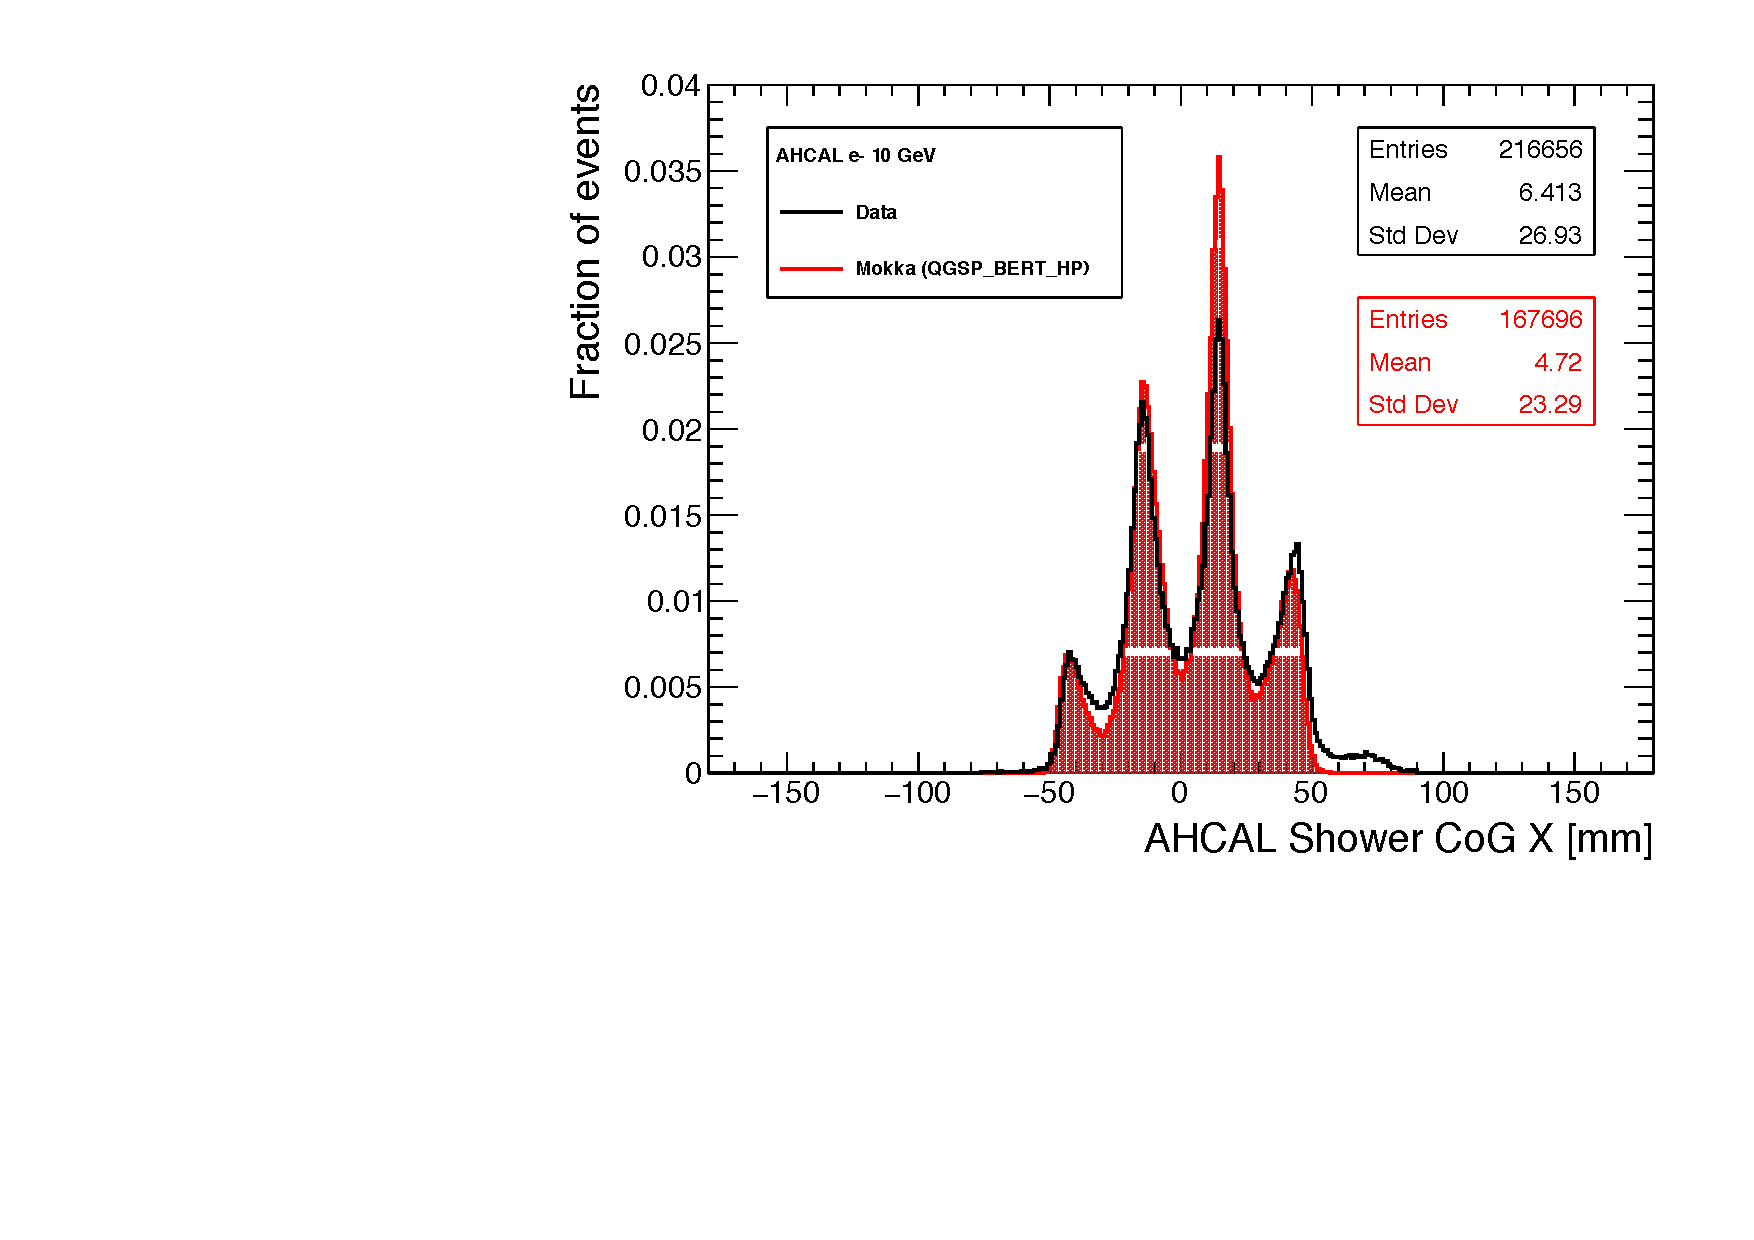
\includegraphics[width=1.\linewidth]{chap5/fig_AHCAL_Timing/Electrons/Run24542_CoGX_AHCAL_10GeV_Comparison.pdf}
    \caption{10 GeV.} \label{fig:e10GeVX}
  \end{subfigure}
  \hfill
  \begin{subfigure}[t]{0.49\textwidth}
    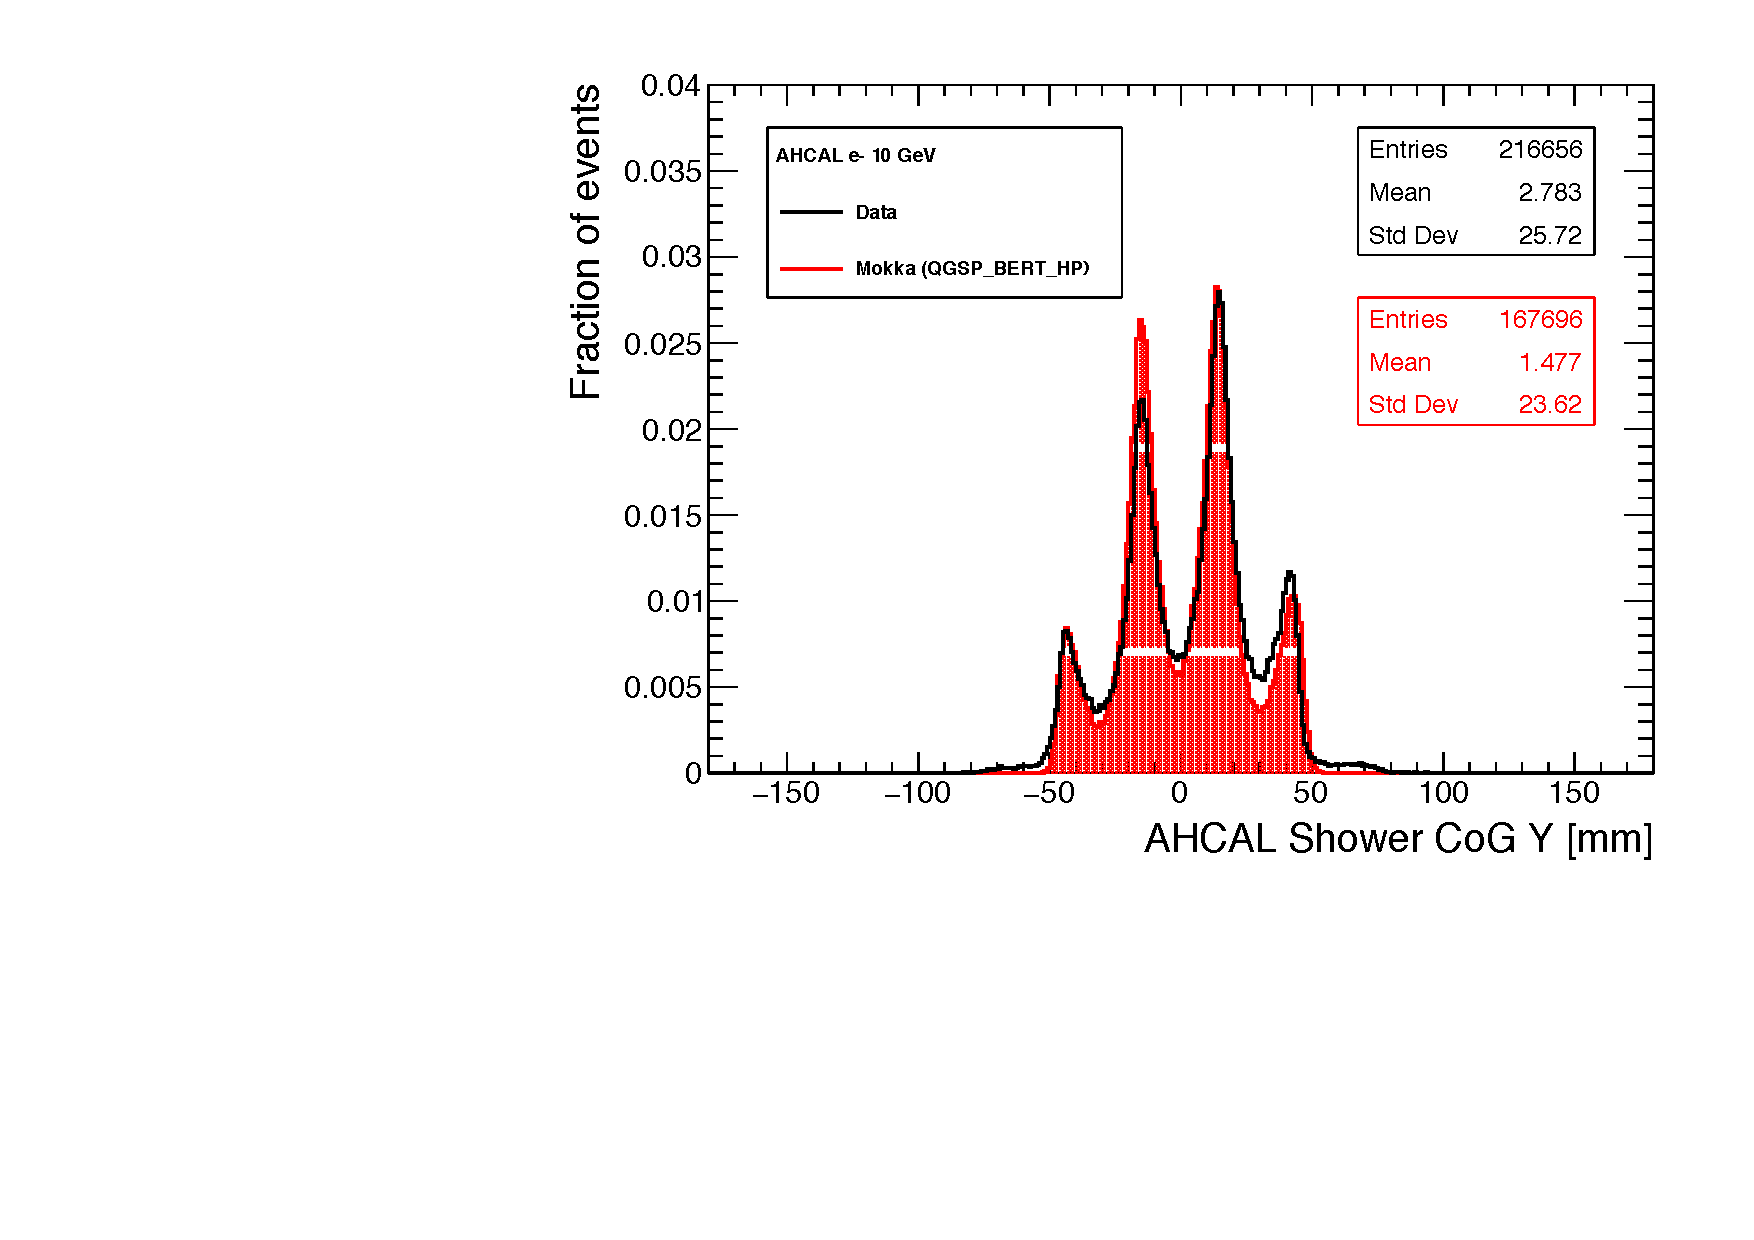
\includegraphics[width=1.\linewidth]{chap5/fig_AHCAL_Timing/Electrons/Run24542_CoGY_AHCAL_10GeV_Comparison.pdf}
    \caption{10 GeV.} \label{fig:e10GeVY}
  \end{subfigure}
  \hfill
  \begin{subfigure}[t]{0.49\textwidth}
    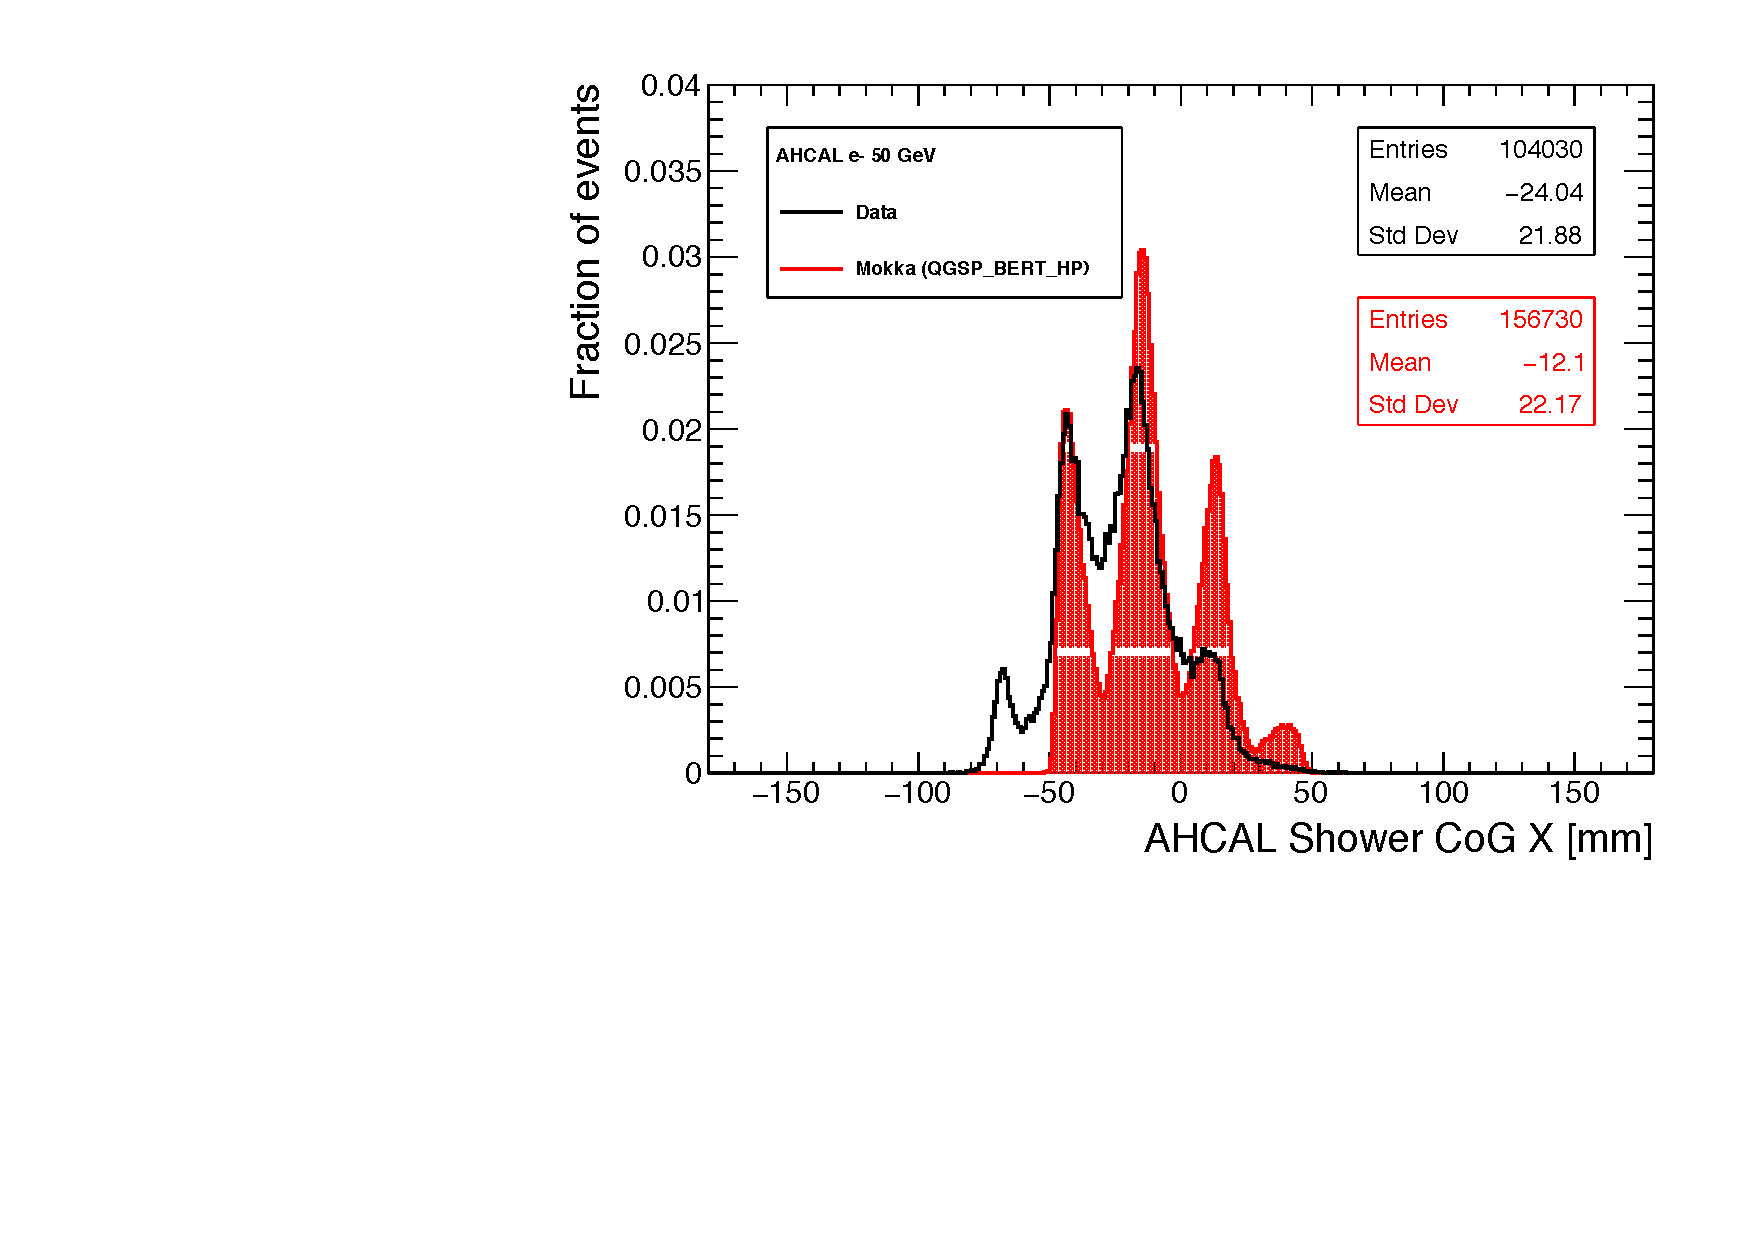
\includegraphics[width=1.\linewidth]{chap5/fig_AHCAL_Timing/Electrons/Run24405_CoGX_AHCAL_50GeV_Comparison.pdf}
    \caption{50 GeV.} \label{fig:e50GeVX}
  \end{subfigure}
  \hfill
  \begin{subfigure}[t]{0.49\textwidth}
    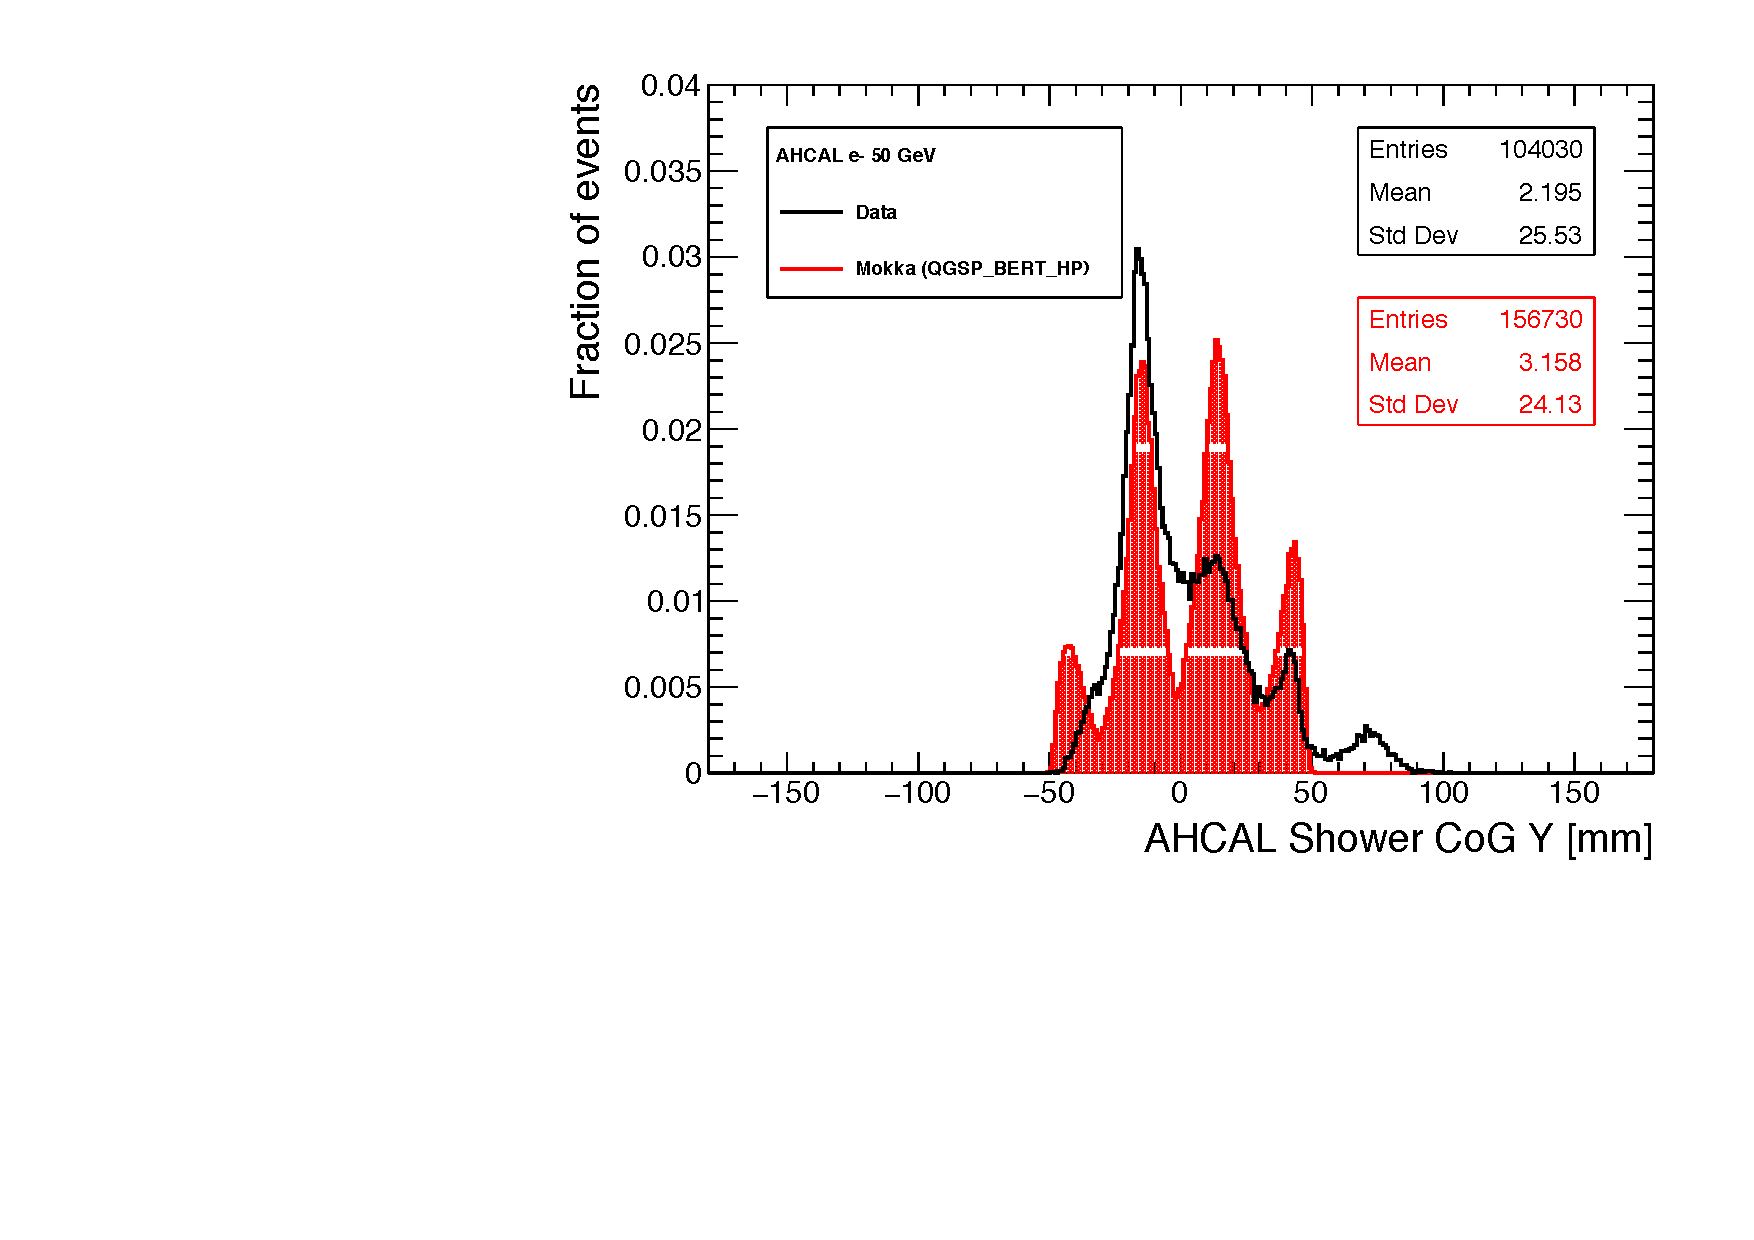
\includegraphics[width=1.\linewidth]{chap5/fig_AHCAL_Timing/Electrons/Run24405_CoGY_AHCAL_50GeV_Comparison.pdf}
    \caption{50 GeV.} \label{fig:e50GeVY}
  \end{subfigure}
  \caption{Beam profiles for 10 GeV and 50 GeV electrons for data and simulation in the x and y directions.}
  \label{fig:BPe}
\end{figure}

\begin{figure}[htbp!]
  \centering
  \begin{subfigure}[t]{0.49\textwidth}
    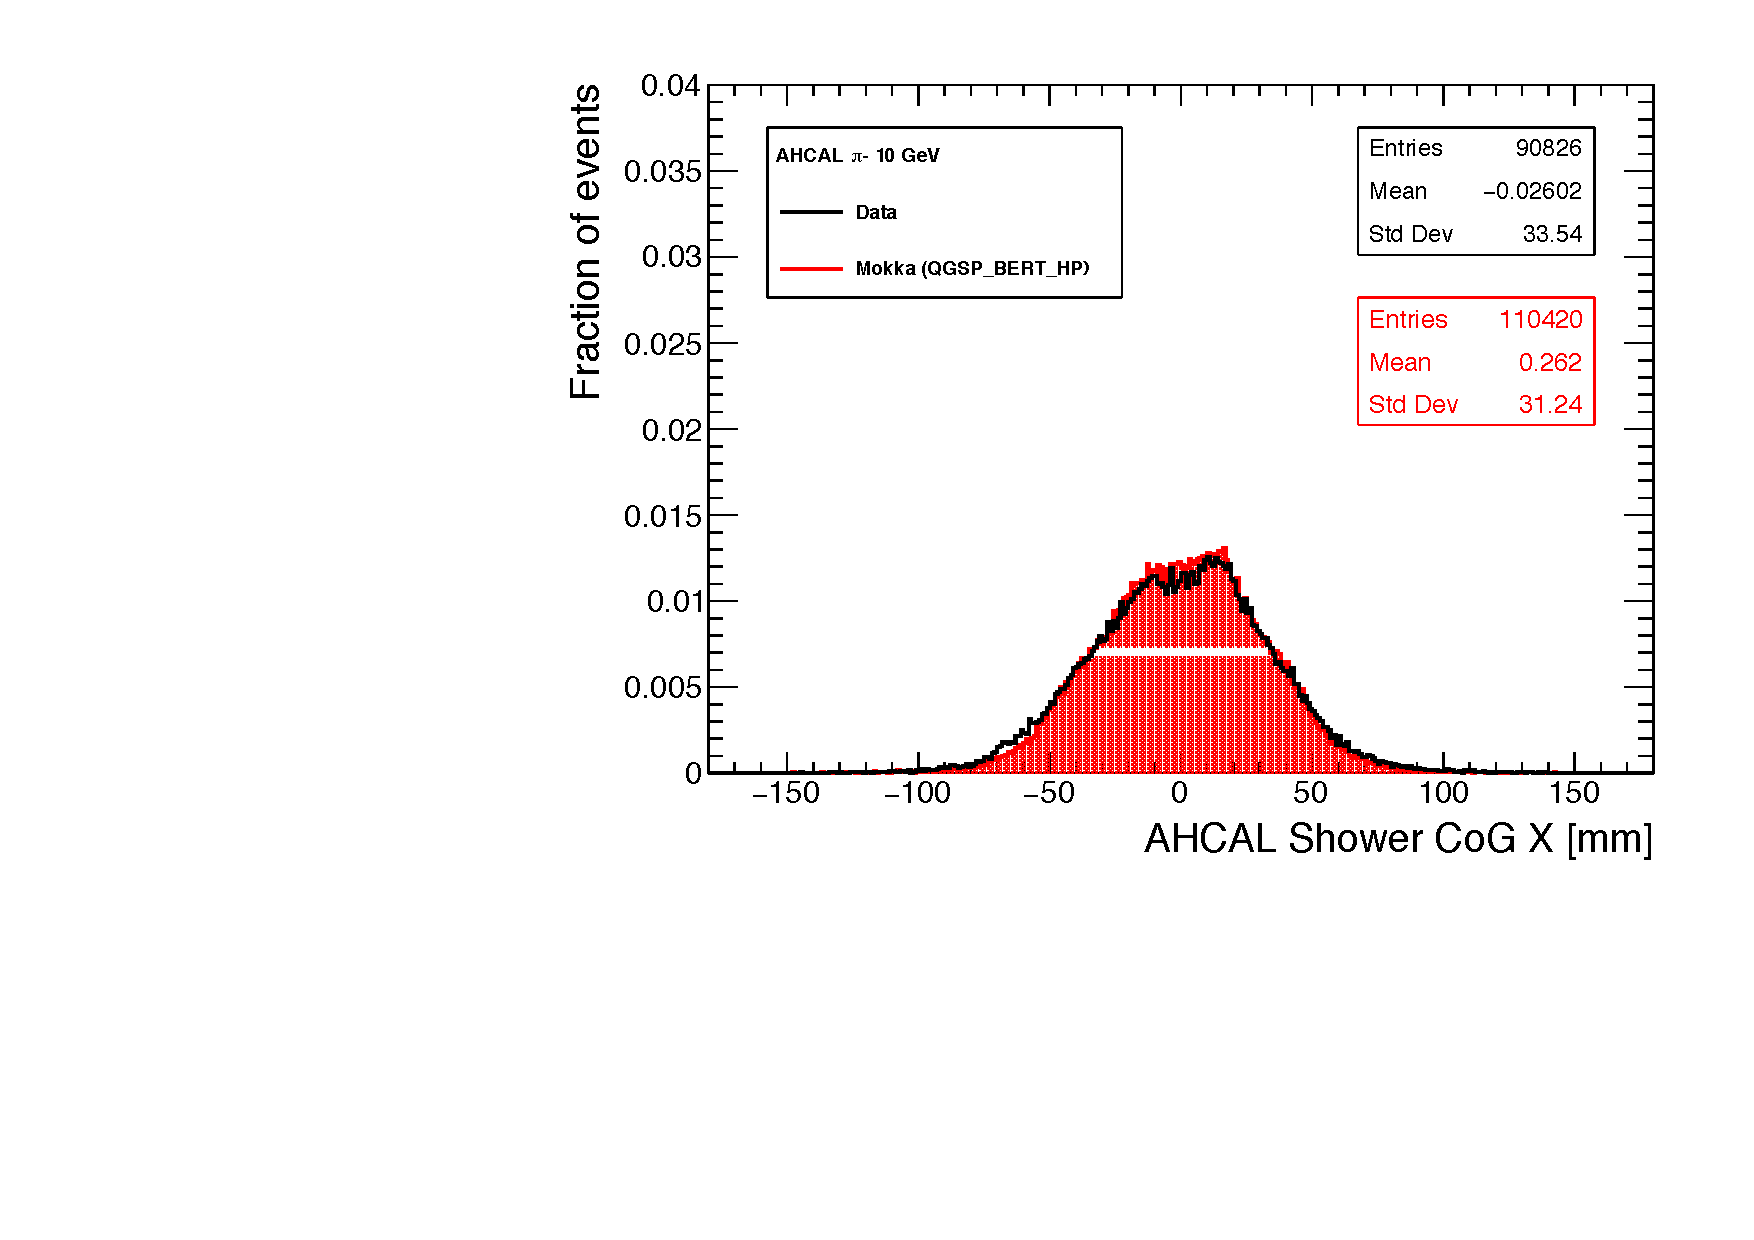
\includegraphics[width=1.\linewidth]{chap5/fig_AHCAL_Timing/Pions/Run24306_CoGX_AHCAL_10GeV_Comparison.pdf}
    \caption{10 GeV.} \label{fig:pi10GeVX}
  \end{subfigure}
  \hfill
  \begin{subfigure}[t]{0.49\textwidth}
    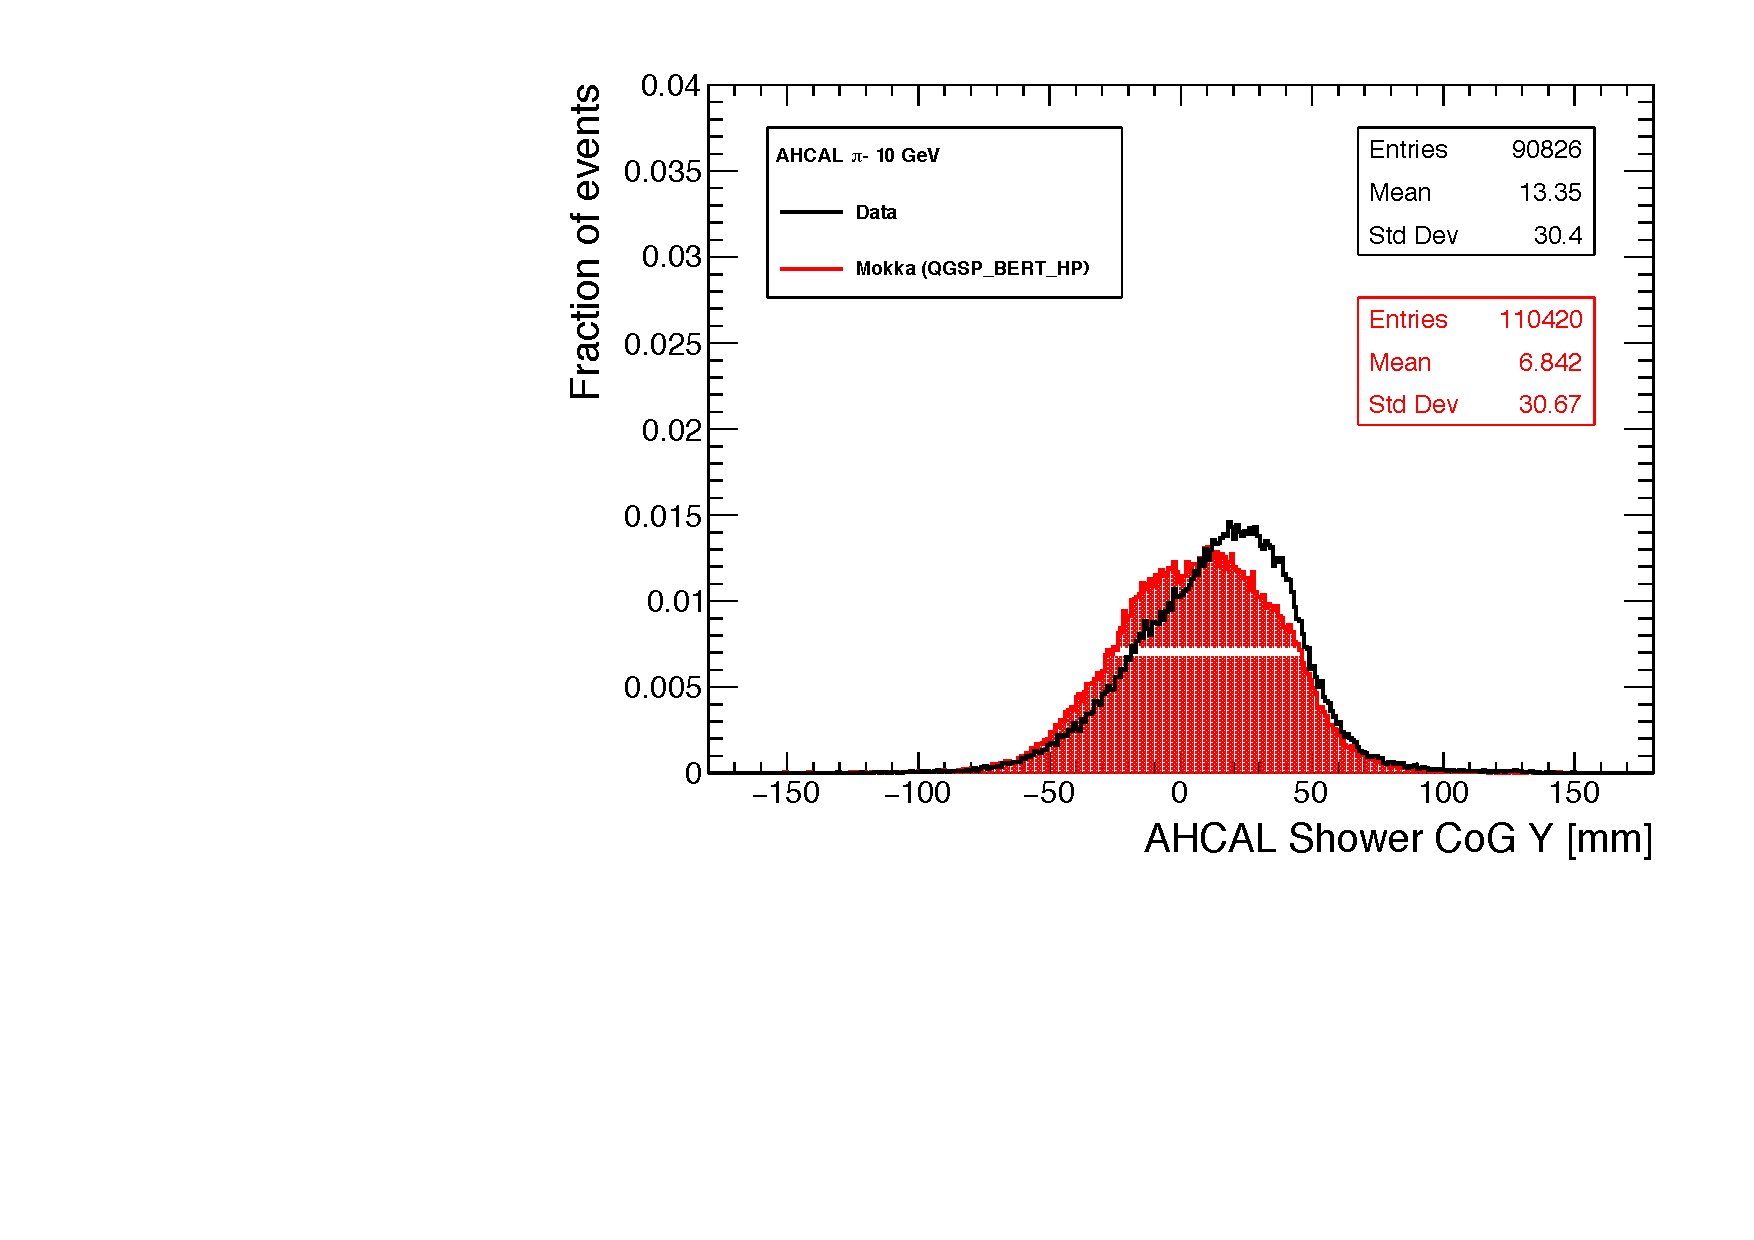
\includegraphics[width=1.\linewidth]{chap5/fig_AHCAL_Timing/Pions/Run24306_CoGY_AHCAL_10GeV_Comparison.pdf}
    \caption{10 GeV.} \label{fig:pi10GeVY}
  \end{subfigure}
  \hfill
  \begin{subfigure}[t]{0.49\textwidth}
    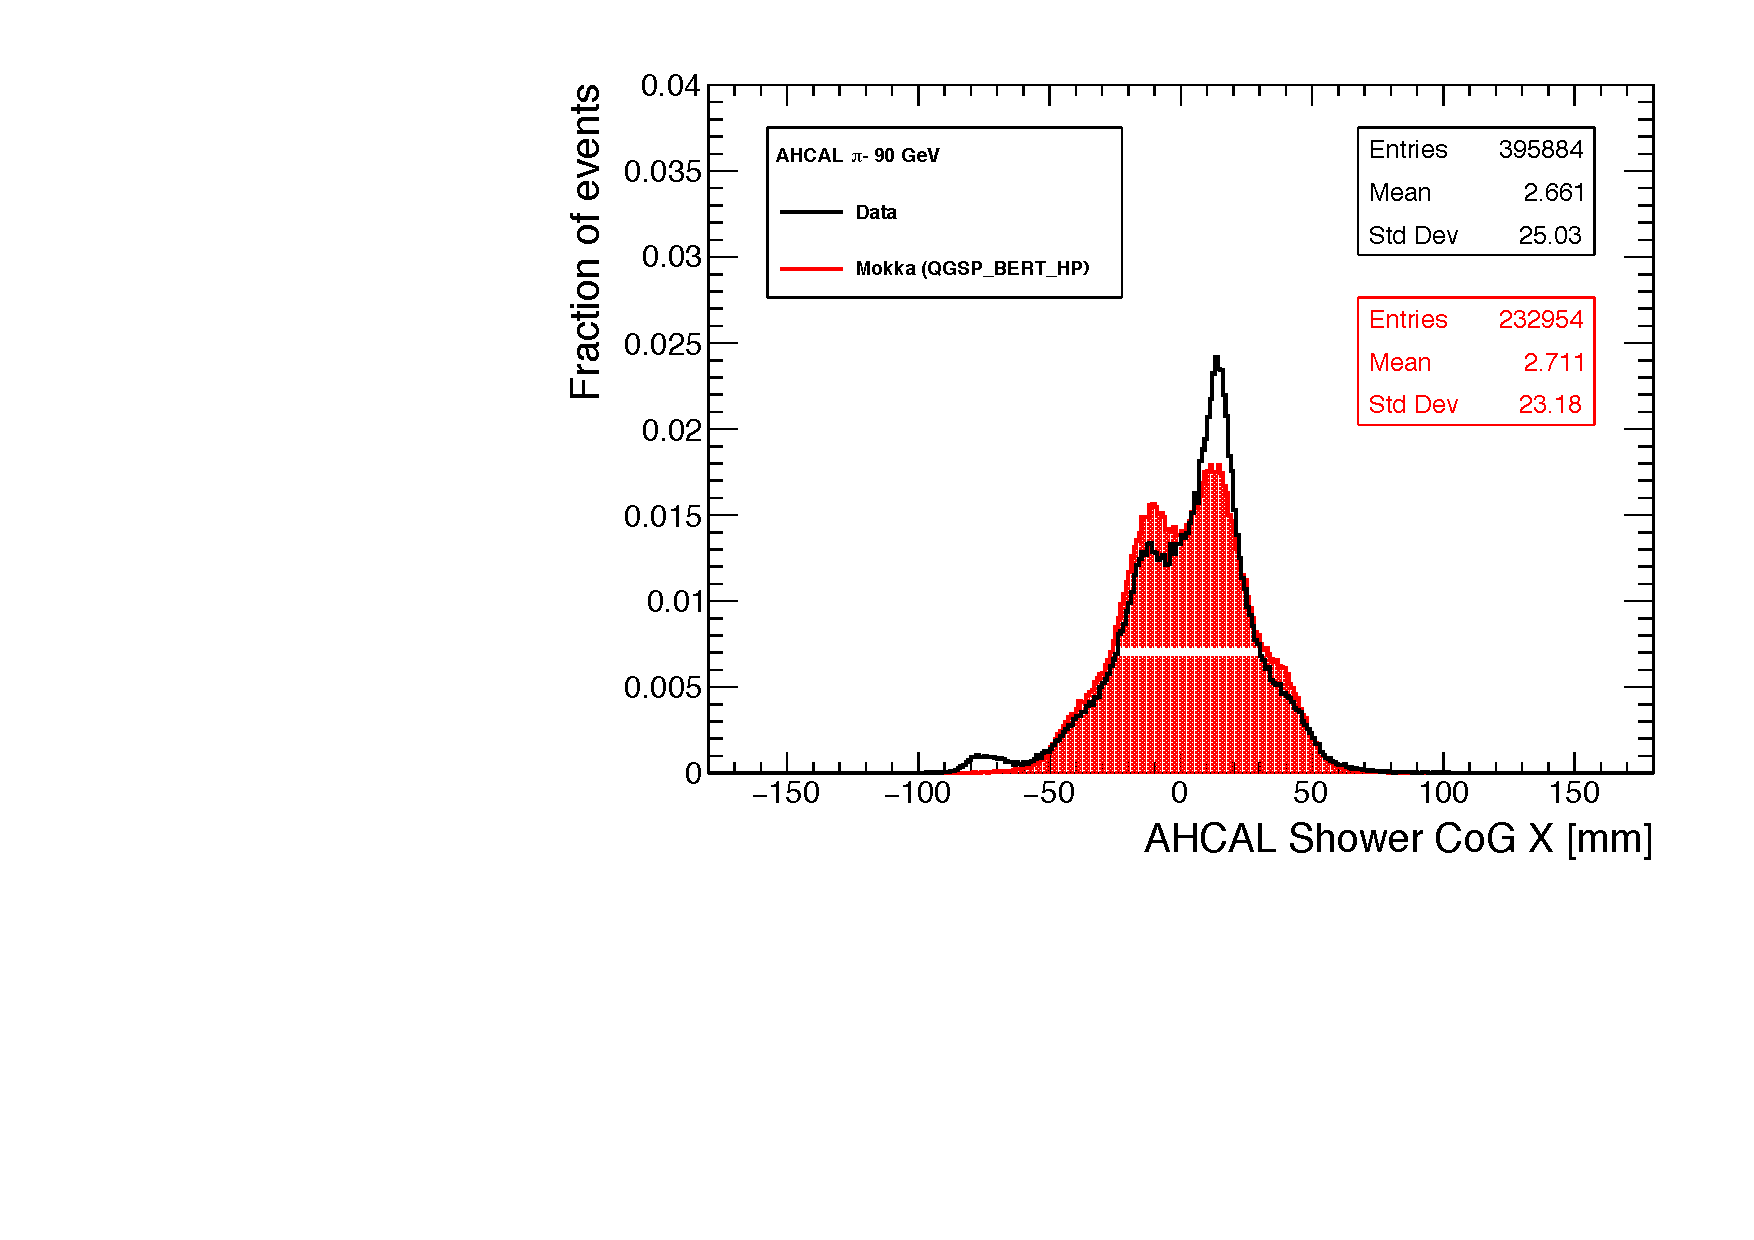
\includegraphics[width=1.\linewidth]{chap5/fig_AHCAL_Timing/Pions/Run24332_CoGX_AHCAL_90GeV_Comparison.pdf}
    \caption{90 GeV.} \label{fig:pi90GeVX}
  \end{subfigure}
  \hfill
  \begin{subfigure}[t]{0.49\textwidth}
    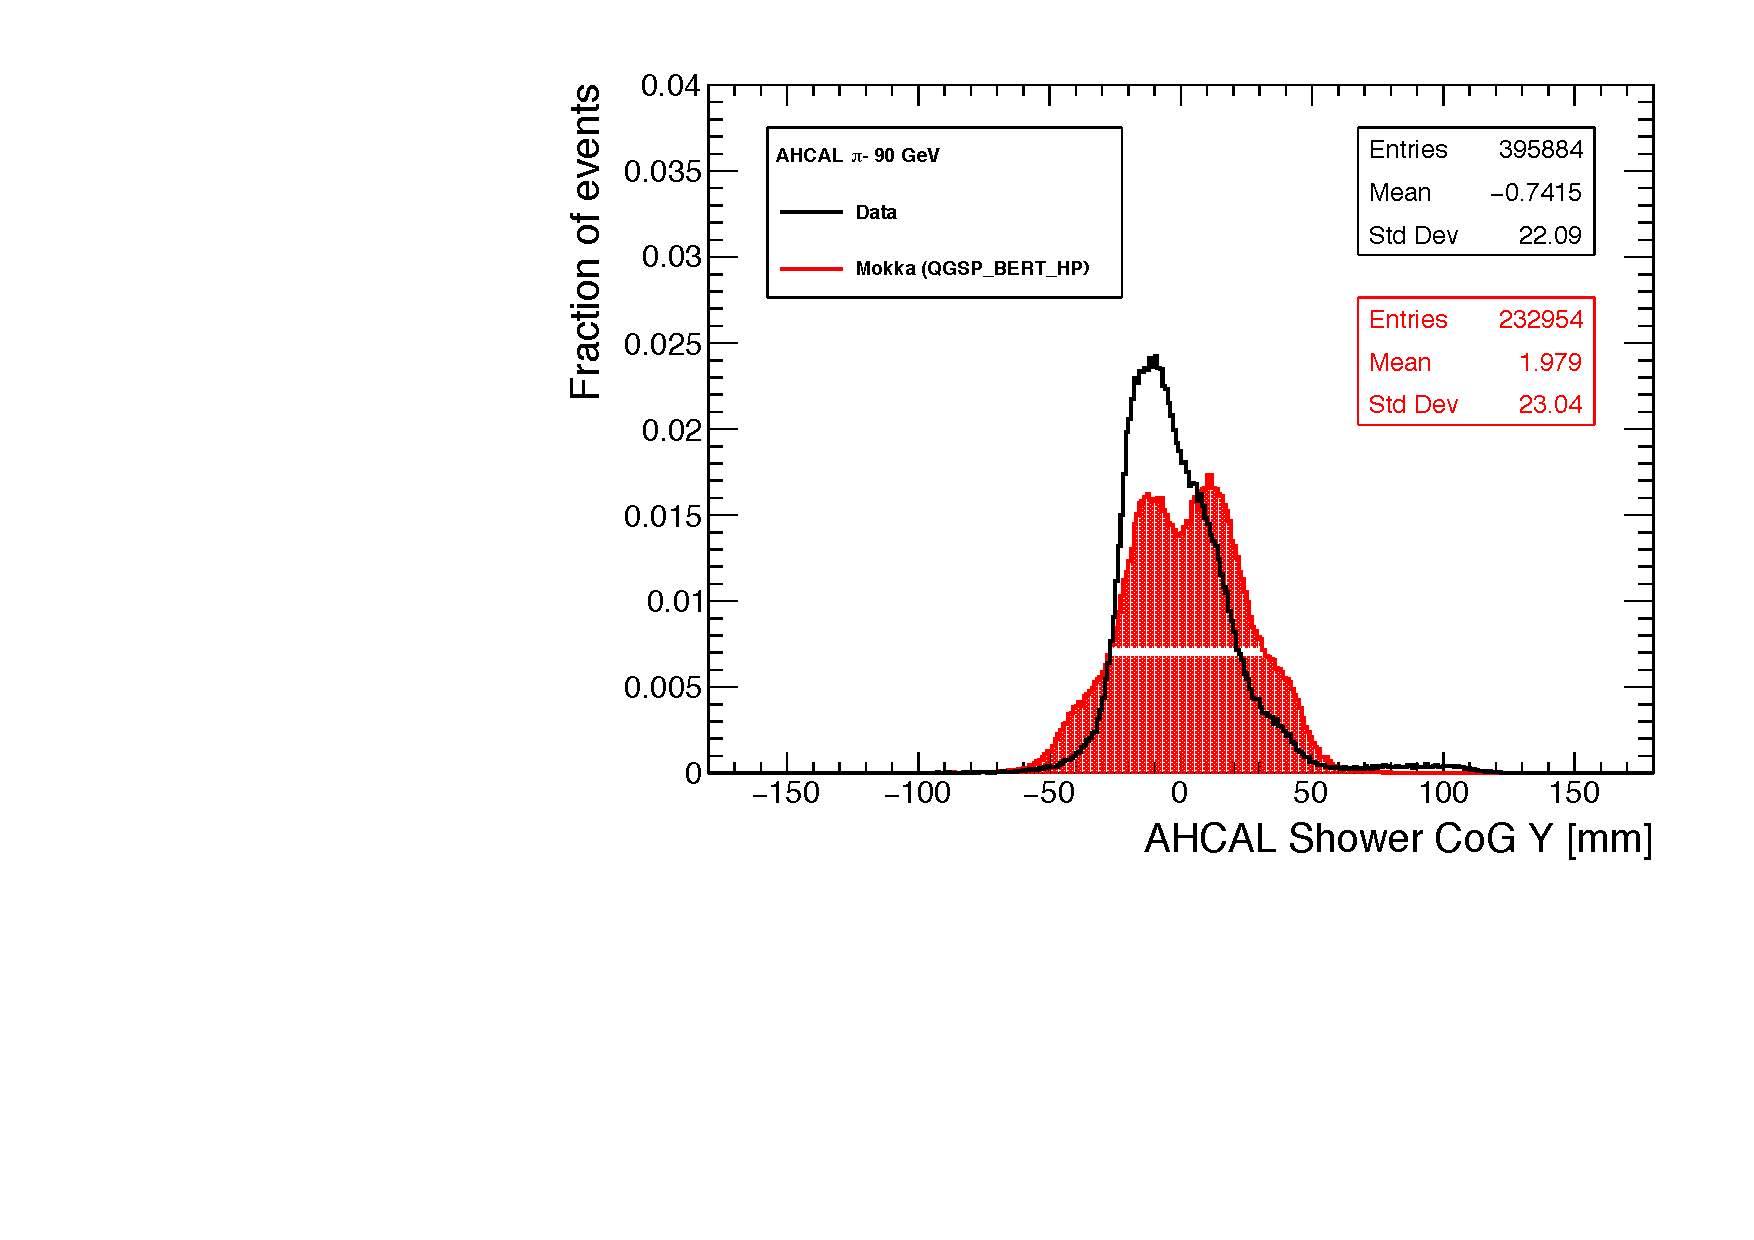
\includegraphics[width=1.\linewidth]{chap5/fig_AHCAL_Timing/Pions/Run24332_CoGY_AHCAL_90GeV_Comparison.pdf}
    \caption{90 GeV.} \label{fig:pi90GeVY}
  \end{subfigure}
  \caption{Beam profiles for 10 GeV and 90 GeV pions for data and simulation in the x and y directions.}
  \label{fig:BPpi}
\end{figure}

\section{Validation of the simulation}

In order to justify any comparison made with the simulation, it needs to be validated first. This is done in two steps using muons and electrons. The comparison of the energy deposited and the number of hits in data and simuation is used to validate the detector simulation. Figures \ref{fig:muVal} show the visible energy $E_{sum}$ and the number of hits above 0.5 MIP for 150 GeV muons in data and simulation.

\begin{figure}[htbp!]
  \centering
  \begin{subfigure}[t]{0.49\textwidth}
    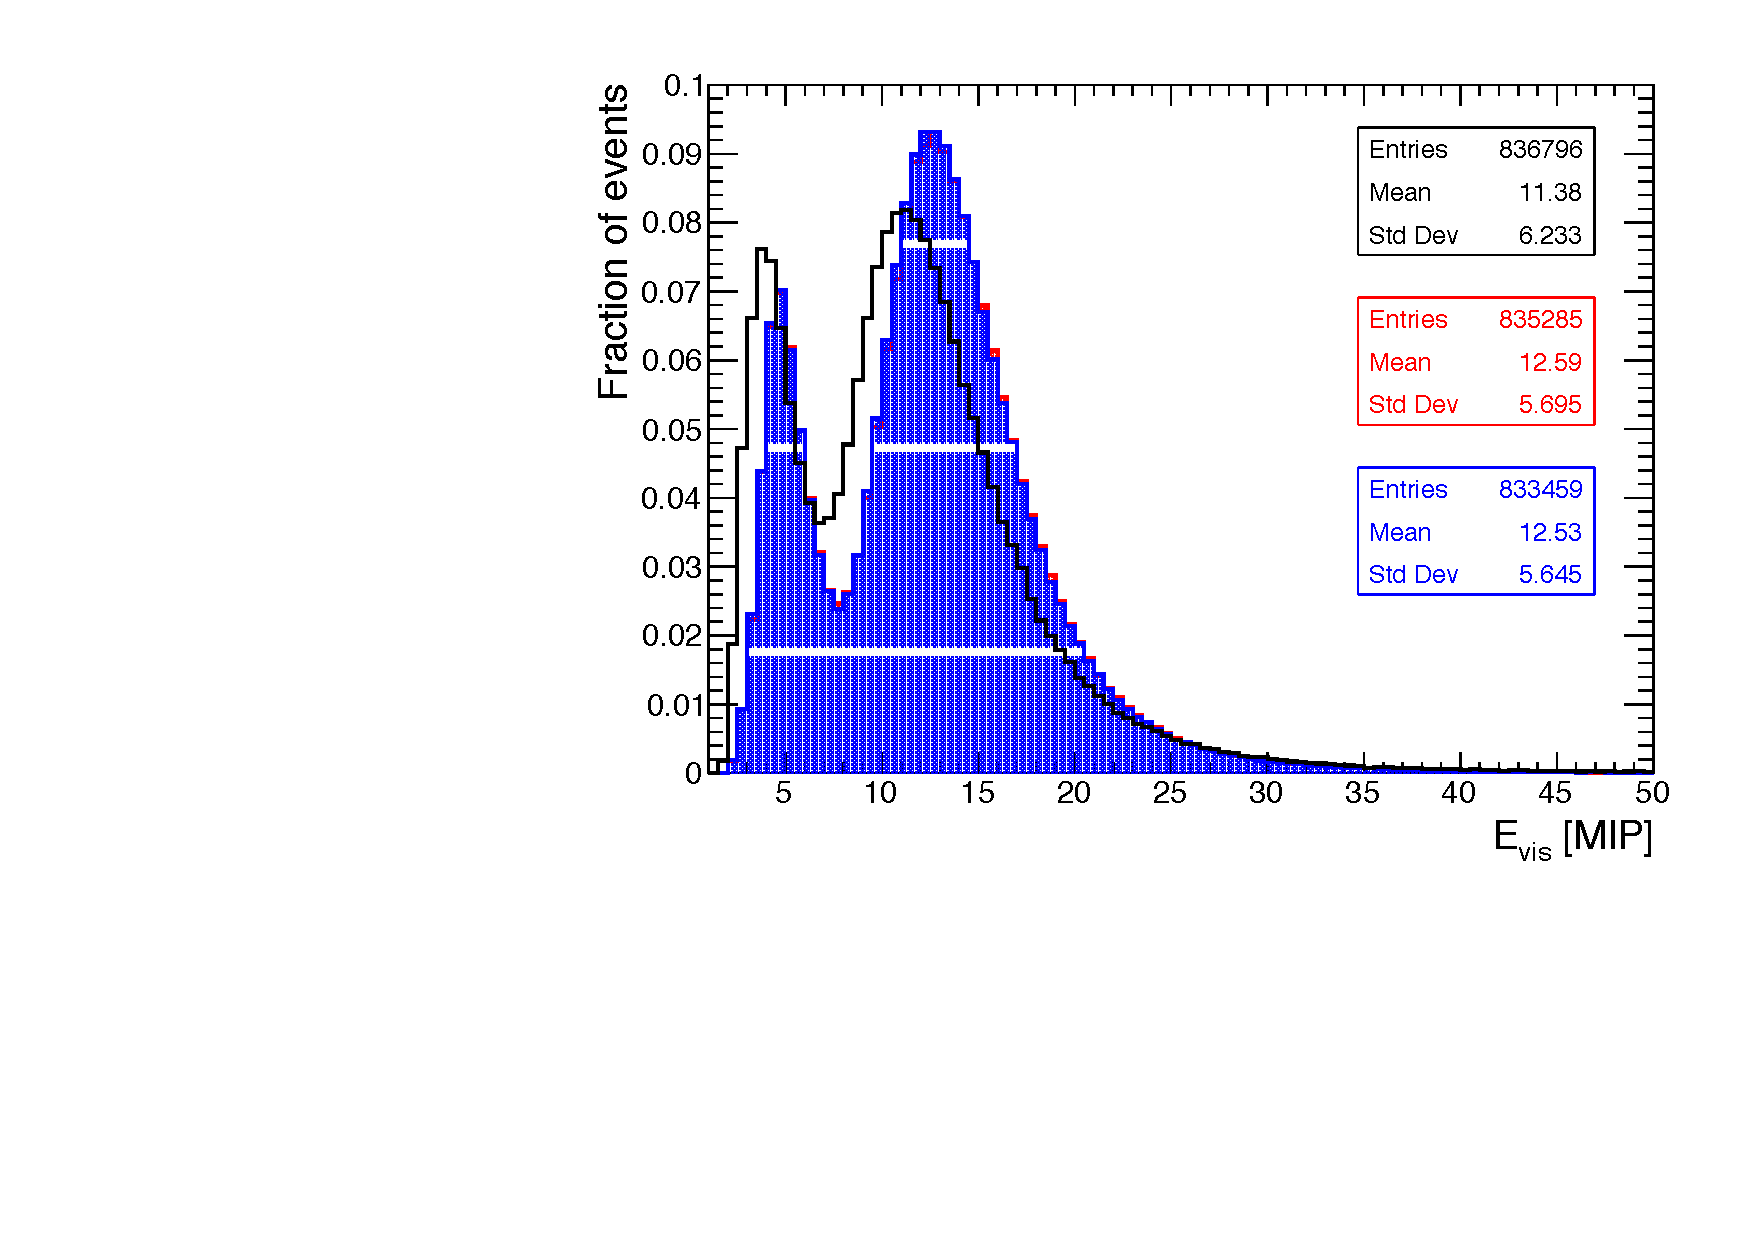
\includegraphics[width=1.\linewidth]{chap5/fig_AHCAL_Timing/Muons/Validation_Evis_Muons.pdf}
    \caption{$E_{sum}$.} \label{fig:muEvis}
  \end{subfigure}
  \hfill
  \begin{subfigure}[t]{0.49\textwidth}
    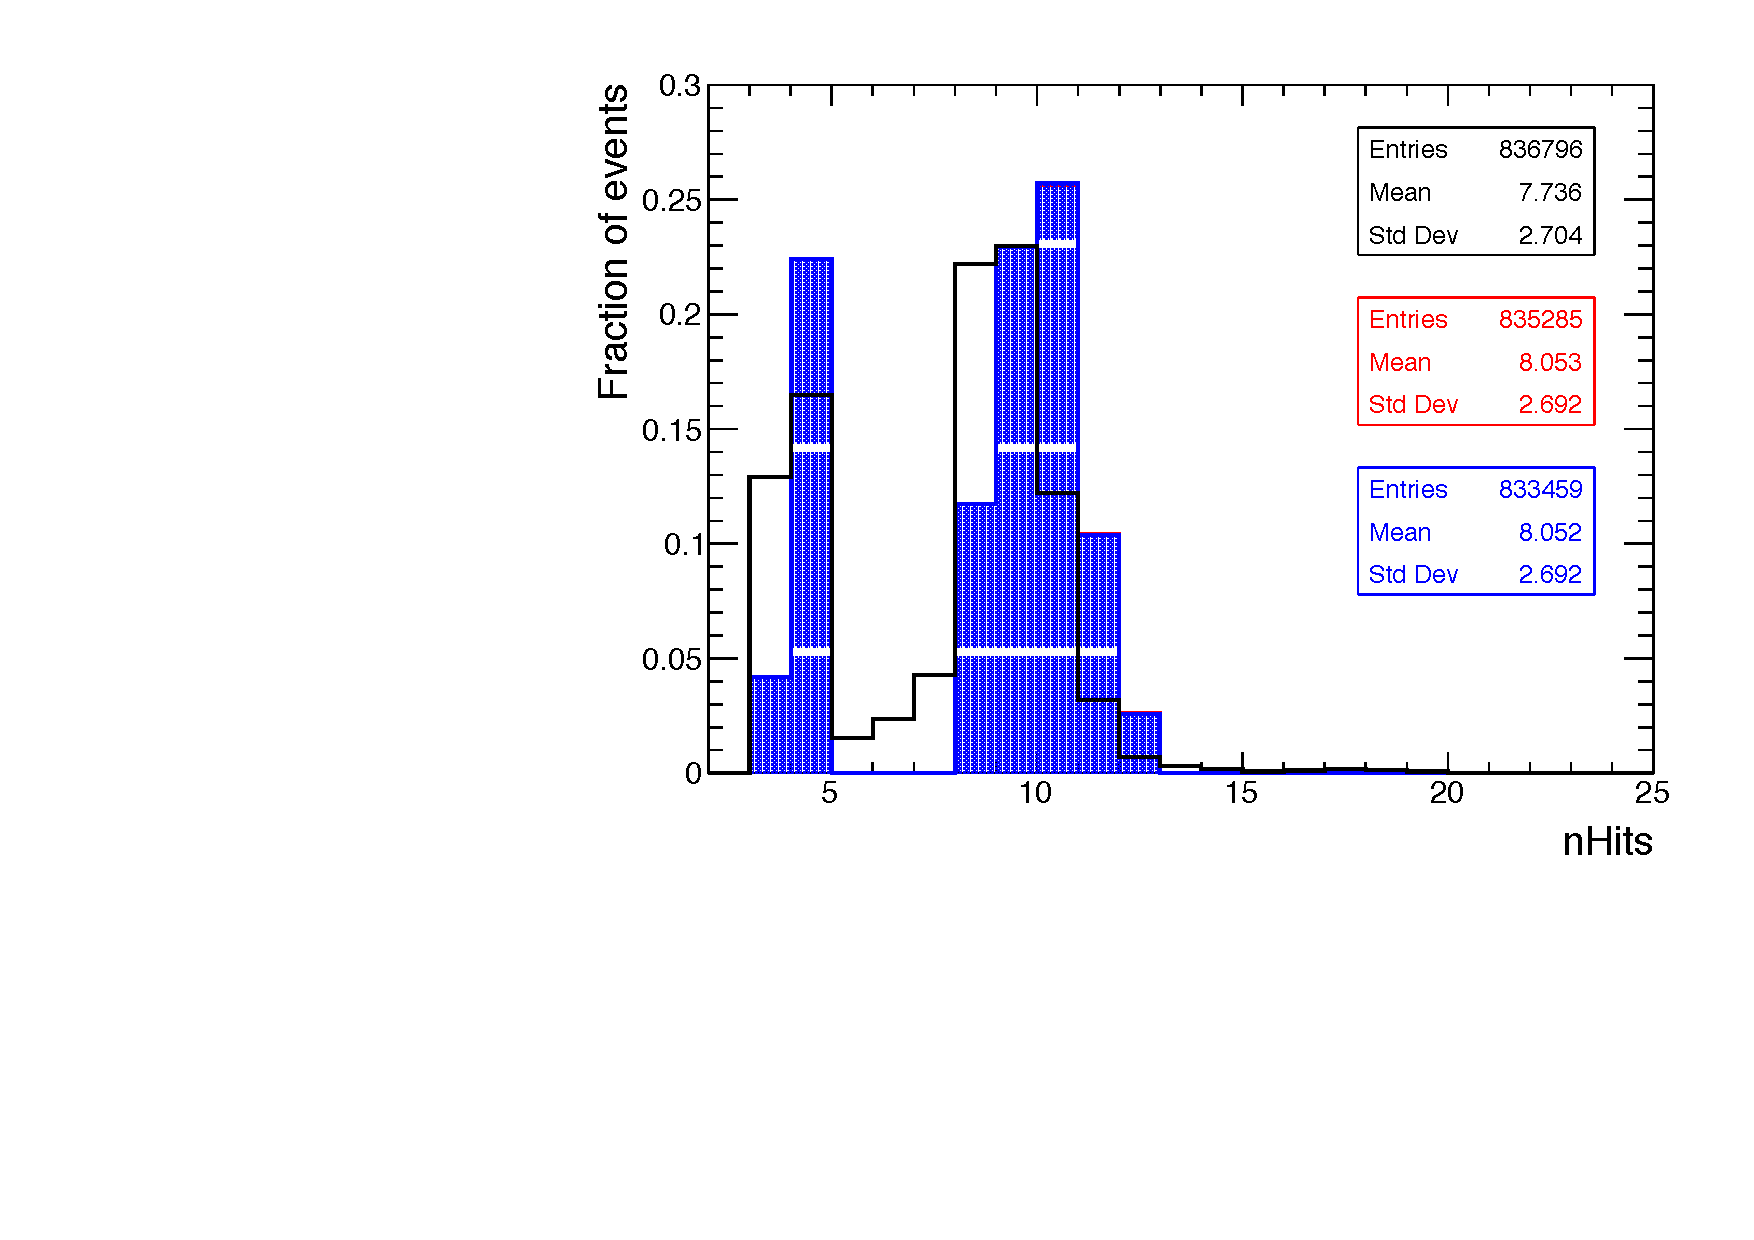
\includegraphics[width=1.\linewidth]{chap5/fig_AHCAL_Timing/Muons/Validation_nHits_Muons.pdf}
    \caption{nHits.} \label{fig:munHits}
  \end{subfigure}
  \caption{\subref{fig:muEvis}) The energy sum in the AHCAL for 150 GeV muons in data and simulations. \subref{fig:munHits}) The number of hits in the AHCAL for 150 GeV muons in data and simulations.}
  \label{fig:muVal}
\end{figure}

One can notice that the distributions are quite similar though the simulation shows a higher mean deposited energy and also less entries to around 5 MIP. As well simulation seems to show a slight higher number of hits. This may be due to the beam profile that is not perfectly well reproduced in simulation. In this case, the impact of dead channels is high depending on where the beam is located. Further, an investigation of the energy deposited per layer has been done and can be seen in figure \ref{fig:muEdep}. It shows that the simulations agree with the data within 5\%. This indicates that the calibration has been performed well for all layers.

\begin{figure}[htbp!]
  \centering
  \begin{subfigure}[t]{0.49\textwidth}
    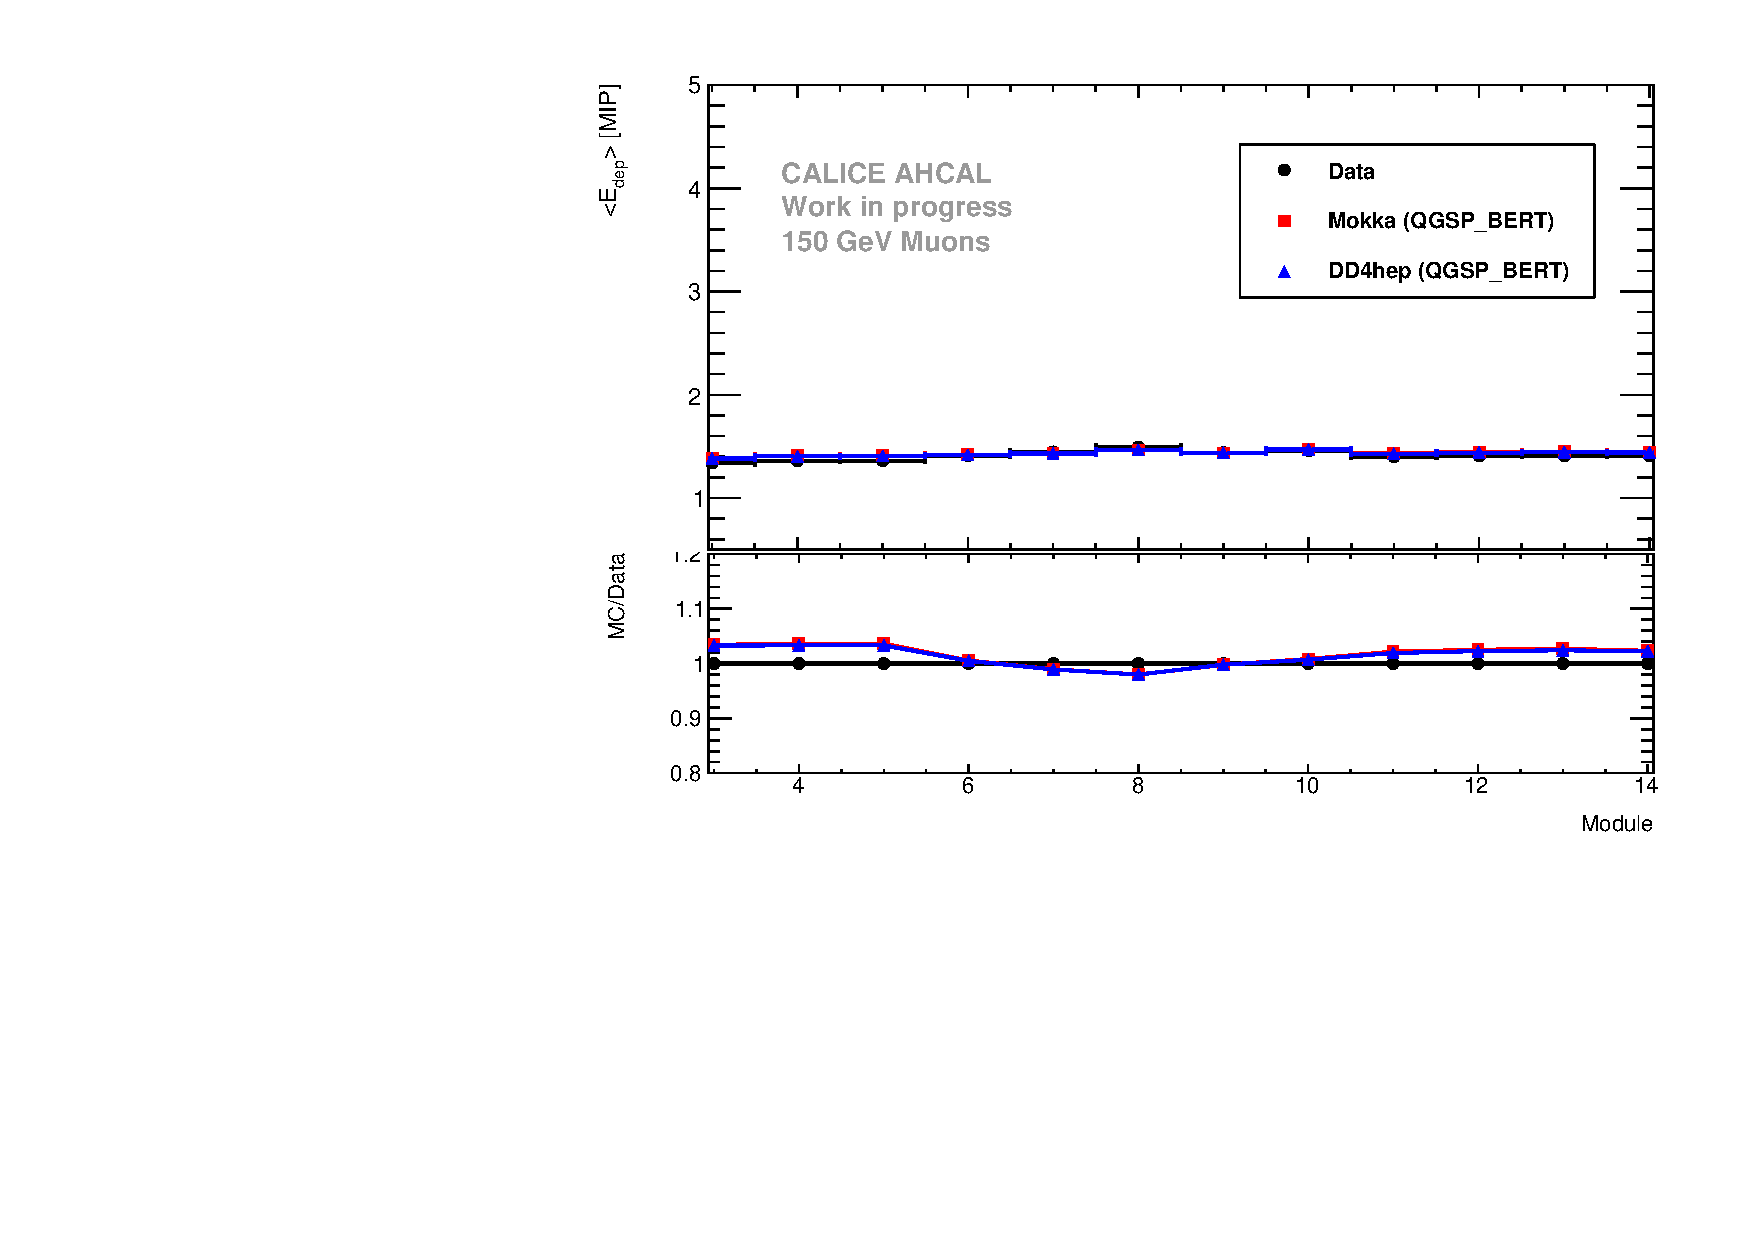
\includegraphics[width=1\linewidth]{chap5/fig_AHCAL_timing/Muons/ProfileMuons_Edep.pdf}
    \caption{} \label{fig:muEdep}
  \end{subfigure}
  \hfill
  \begin{subfigure}[t]{0.49\textwidth}
    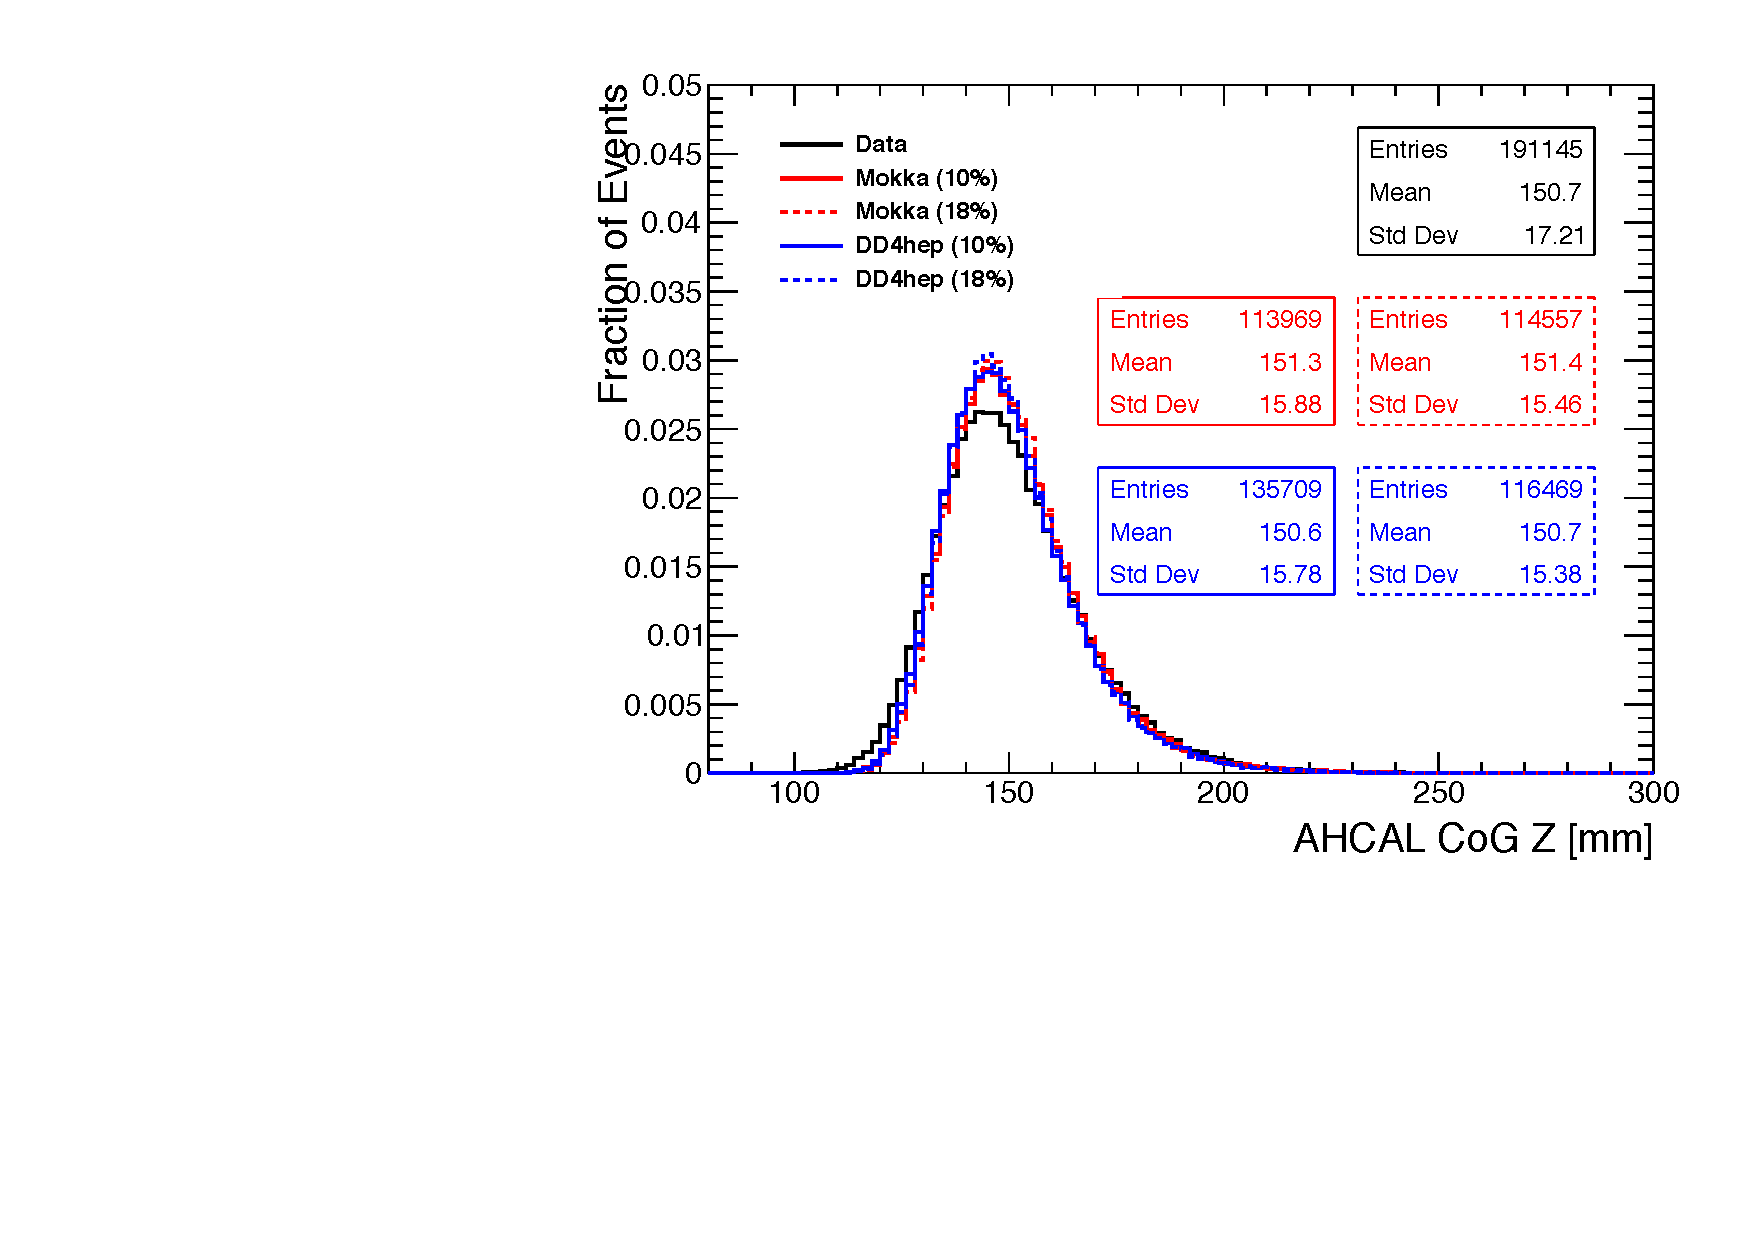
\includegraphics[width=1.\linewidth]{chap5/fig_AHCAL_Timing/Electrons/Comparison_CoGZ_Xtalk_electrons10GeV.pdf}
    \caption{} \label{fig:e10GoGZ}
  \end{subfigure}
  \caption{\subref{fig:muEdep}) Longitudinal energy profile for 150 GeV muons for data and simulations. \subref{fig:e10GoGZ}) Distribution of the center of gravity in the z direction for 10 GeV electrons for data and simulation.}
  \label{fig:Val}
\end{figure}

In a second part, electrons are used to validate further the simulation. As the physics of electron showers is very well understood and can be simulated with great accuracy, it is used as a tool to validate the detector geometry especially concerning the material budget. Also besides noise and beam profiles, the influence of cross-talk has a significant impact due to the higher energy deposited. Moreover, desaturation of high energy cells is very important as generally electrons deposit in few cells their energy. Unfortunately no saturation curves are available and only estimations of the necessary parameters are derived from simulation by tuning it to the data. Though, in this analysis, the energy deposited in a single cell is only relevant at low energies (from 0.5 to few MIPs) where the response of the SiPM is linear. Thus desaturation is not used. Simple shower variables have been looked at such as number of hits, energy sum and center of gravity in z direction per event in order to validate the simulation.

The center of gravity in z was looked at as this variable is mostly sensible to the amount of material upstream to the calorimter. The figure \ref{fig:e10GoGZ} shows that the data and simulations agree rather well despite the data seems to shower slightly before. Figures \ref{fig:e10Val} and \ref{fig:e50Val} show the distribution of the energy sum $E_{sum}$ in the AHCAL and the number of hits $nHits$ for 10 GeV and 50 GeV electrons for data and simulations. Two different version of the simulations, with a cross-talk parameter of 10\% or 18\% are shown. For 10 GeV, 10\% cross-talk seems better whereas for 50 GeV, the value of 18\% seems favored. A value of 15\% was chosen for the simulation as neither neither simulations fit the data for both observables. One can also notice that for 50 GeV, a large tail to the left of both distributions is visible. This has been investigated in details \cite{AmbraEnergy}, but the origin of this is still not clear and may come from contamination from lower energy electrons. This is not a problem in itself for this analysis as only timing is investigated.

\begin{figure}[htbp!]
  \centering
  \begin{subfigure}[t]{0.49\textwidth}
    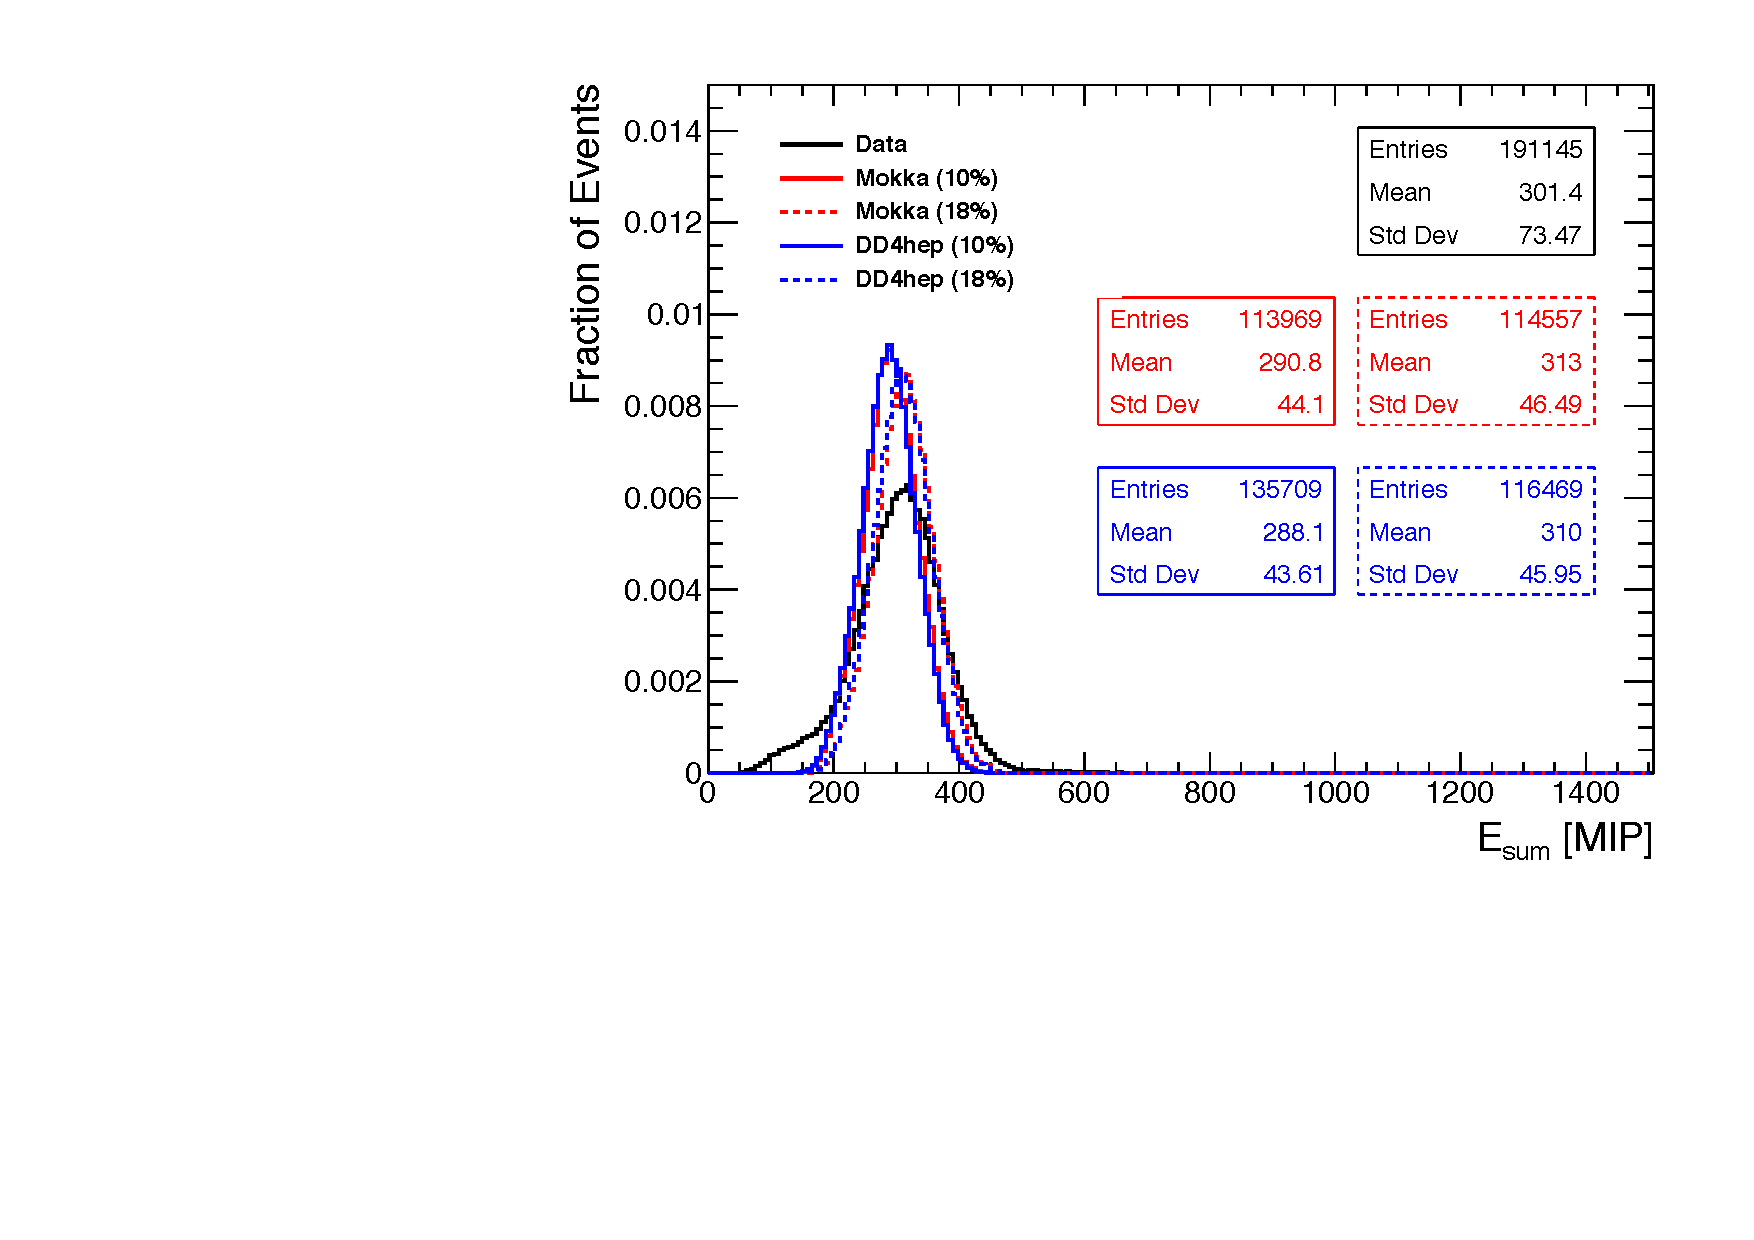
\includegraphics[width=1.\linewidth]{chap5/fig_AHCAL_Timing/Electrons/Comparison_EnergySum_Xtalk_electrons10GeV.pdf}
    \caption{$E_{sum}$.} \label{fig:e10Evis}
  \end{subfigure}
  \hfill
  \begin{subfigure}[t]{0.49\textwidth}
    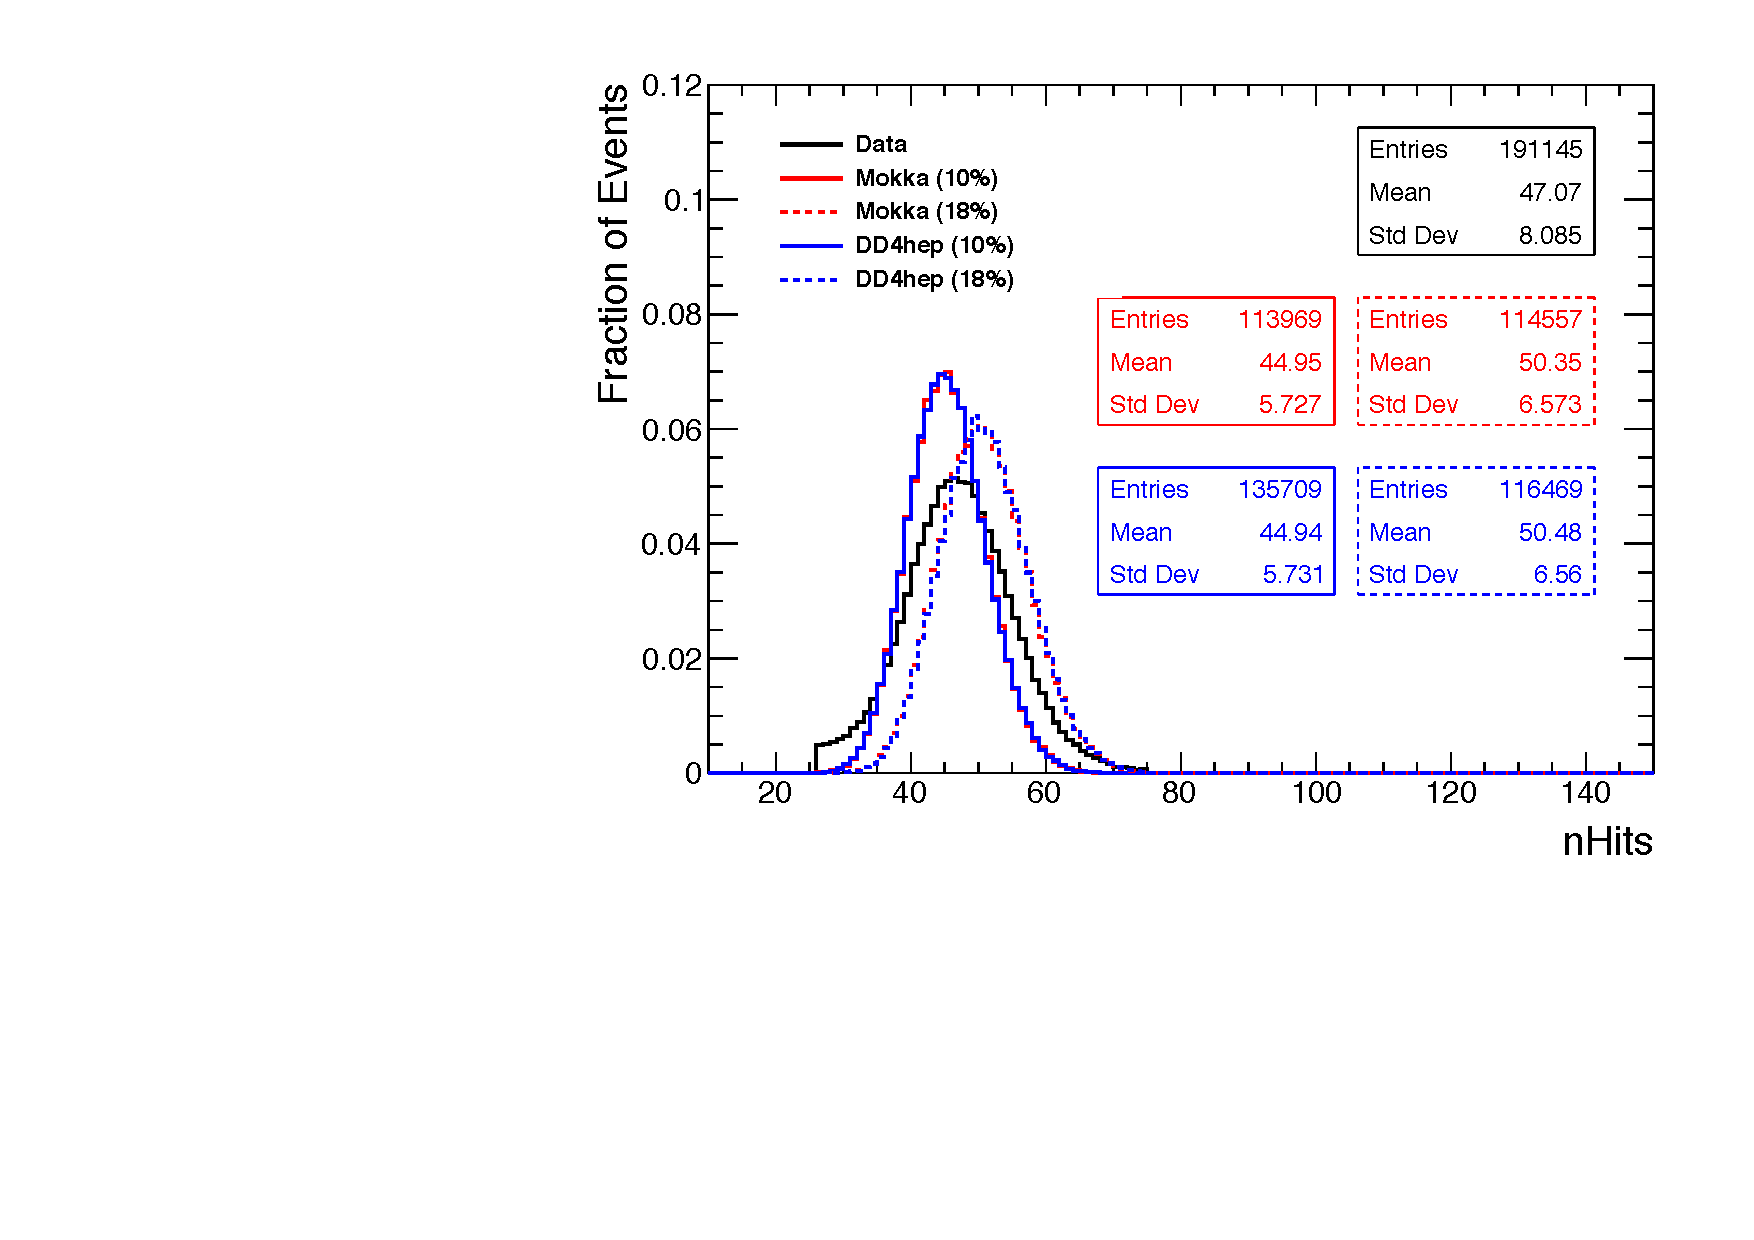
\includegraphics[width=1.\linewidth]{chap5/fig_AHCAL_Timing/Electrons/Comparison_nHits_Xtalk_electrons10GeV.pdf}
    \caption{nHits.} \label{fig:e10nHits}
  \end{subfigure}
  \caption{\subref{fig:e10Evis}) The energy sum in the AHCAL for 10 GeV electrons for data and simulations with a cross-talk value of 10\% and 18\%. \subref{fig:e10nHits}) The number of hits in the AHCAL for 10 GeV electrons for data and simulations with a cross-talk value of 10\% and 18\%.}
  \label{fig:e10Val}
\end{figure}

\begin{figure}[htbp!]
  \centering
  \begin{subfigure}[t]{0.49\textwidth}
    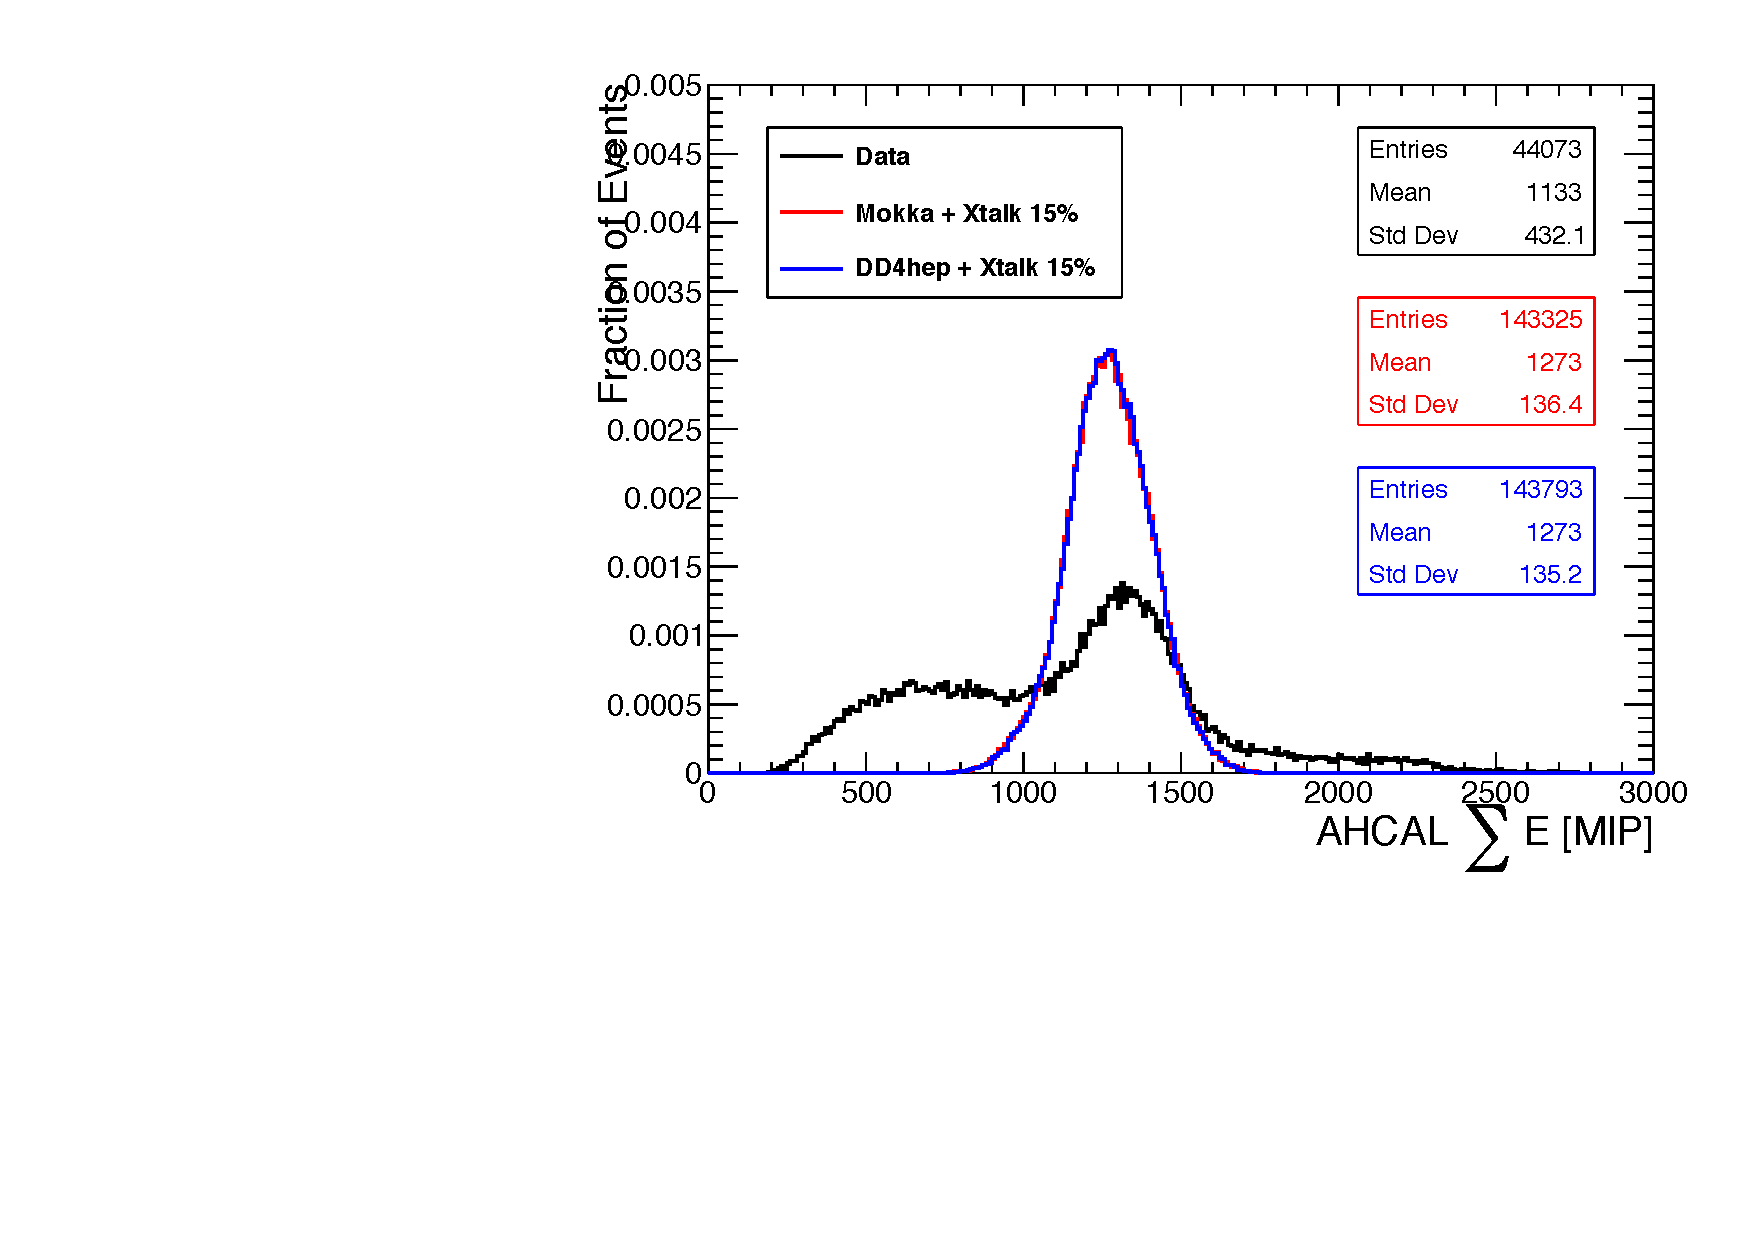
\includegraphics[width=1.\linewidth]{chap5/fig_AHCAL_Timing/Electrons/Comparison_EnergySum_Xtalk_electrons50GeV.pdf}
    \caption{$E_{sum}$.} \label{fig:e50Evis}
  \end{subfigure}
  \hfill
  \begin{subfigure}[t]{0.49\textwidth}
    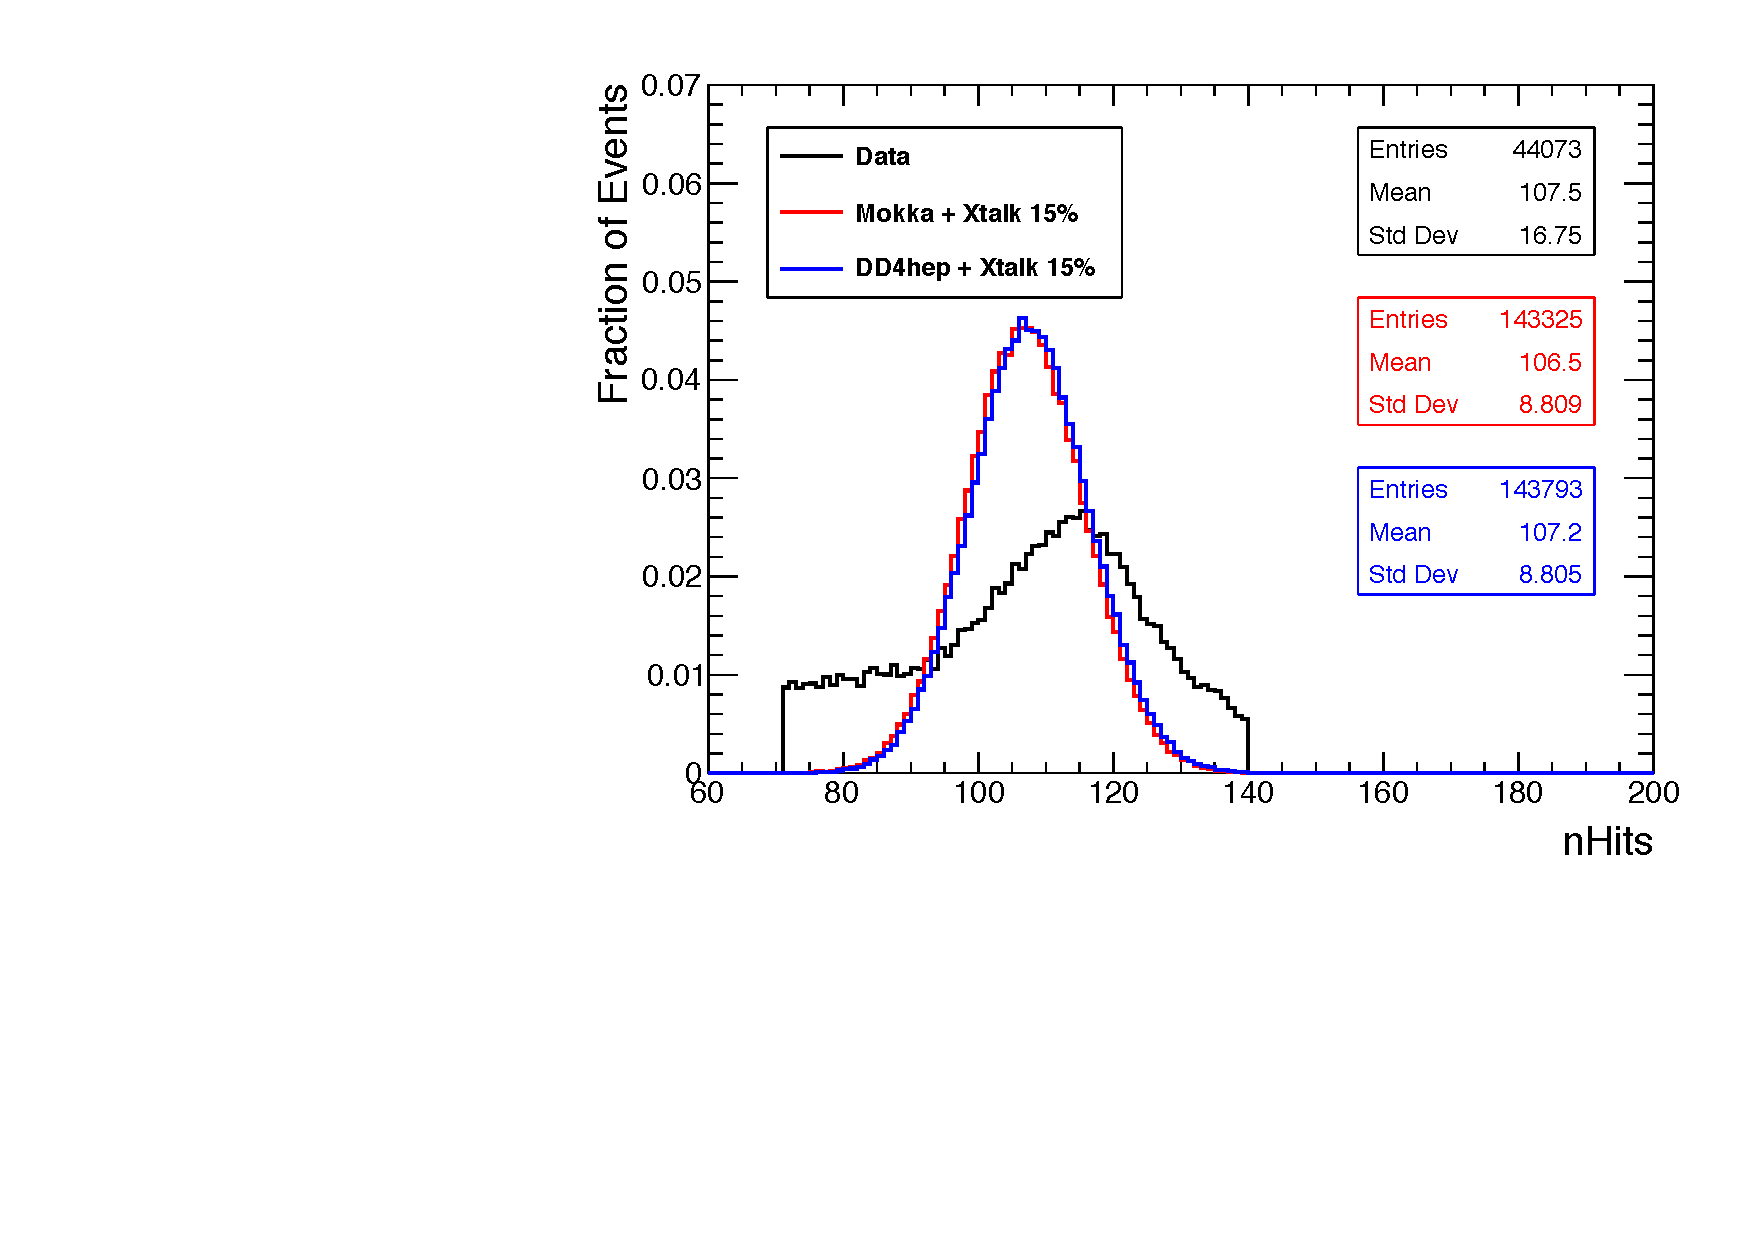
\includegraphics[width=1.\linewidth]{chap5/fig_AHCAL_Timing/Electrons/Comparison_nHits_Xtalk_electrons50GeV.pdf}
    \caption{nHits.} \label{fig:e50nHits}
  \end{subfigure}
  \caption{\subref{fig:e50Evis}) The energy sum in the AHCAL for 50 GeV electrons for data and simulations with a cross-talk value of 10\% and 18\%. \subref{fig:e50nHits}) The number of hits in the AHCAL for 50 GeV electrons for data and simulations with a cross-talk value of 10\% and 18\%.}
  \label{fig:e50Val}
\end{figure}

Figures \ref{fig:eVal} show the mean energy sum $<E_{sum}>$ and mean number of hits $<nHits>$ as function of the electron beam energy between 10 and 50 GeV for data and simulation with different cross-talk parameters. The visible energy for data agrees within the simulations for 10, 15 and 20 GeV electron energy and seems to agree better with the 10\% cross-talk simulations. For higher energies, the data deviates significantly to lower values due to the presence of the long tail left of the distribution that the simulations cannot describe. The number of hits is well described, certainly due to the selection cut on the number of hits, with the simulations but agrees better with 10\% at low energies and with the 18\% at higher energies. However, the data cannot be described for both distributions at once in either simulations with a global cross-talk parameter.

\begin{figure}[htbp!]
  \centering
  \begin{subfigure}[t]{0.49\textwidth}
    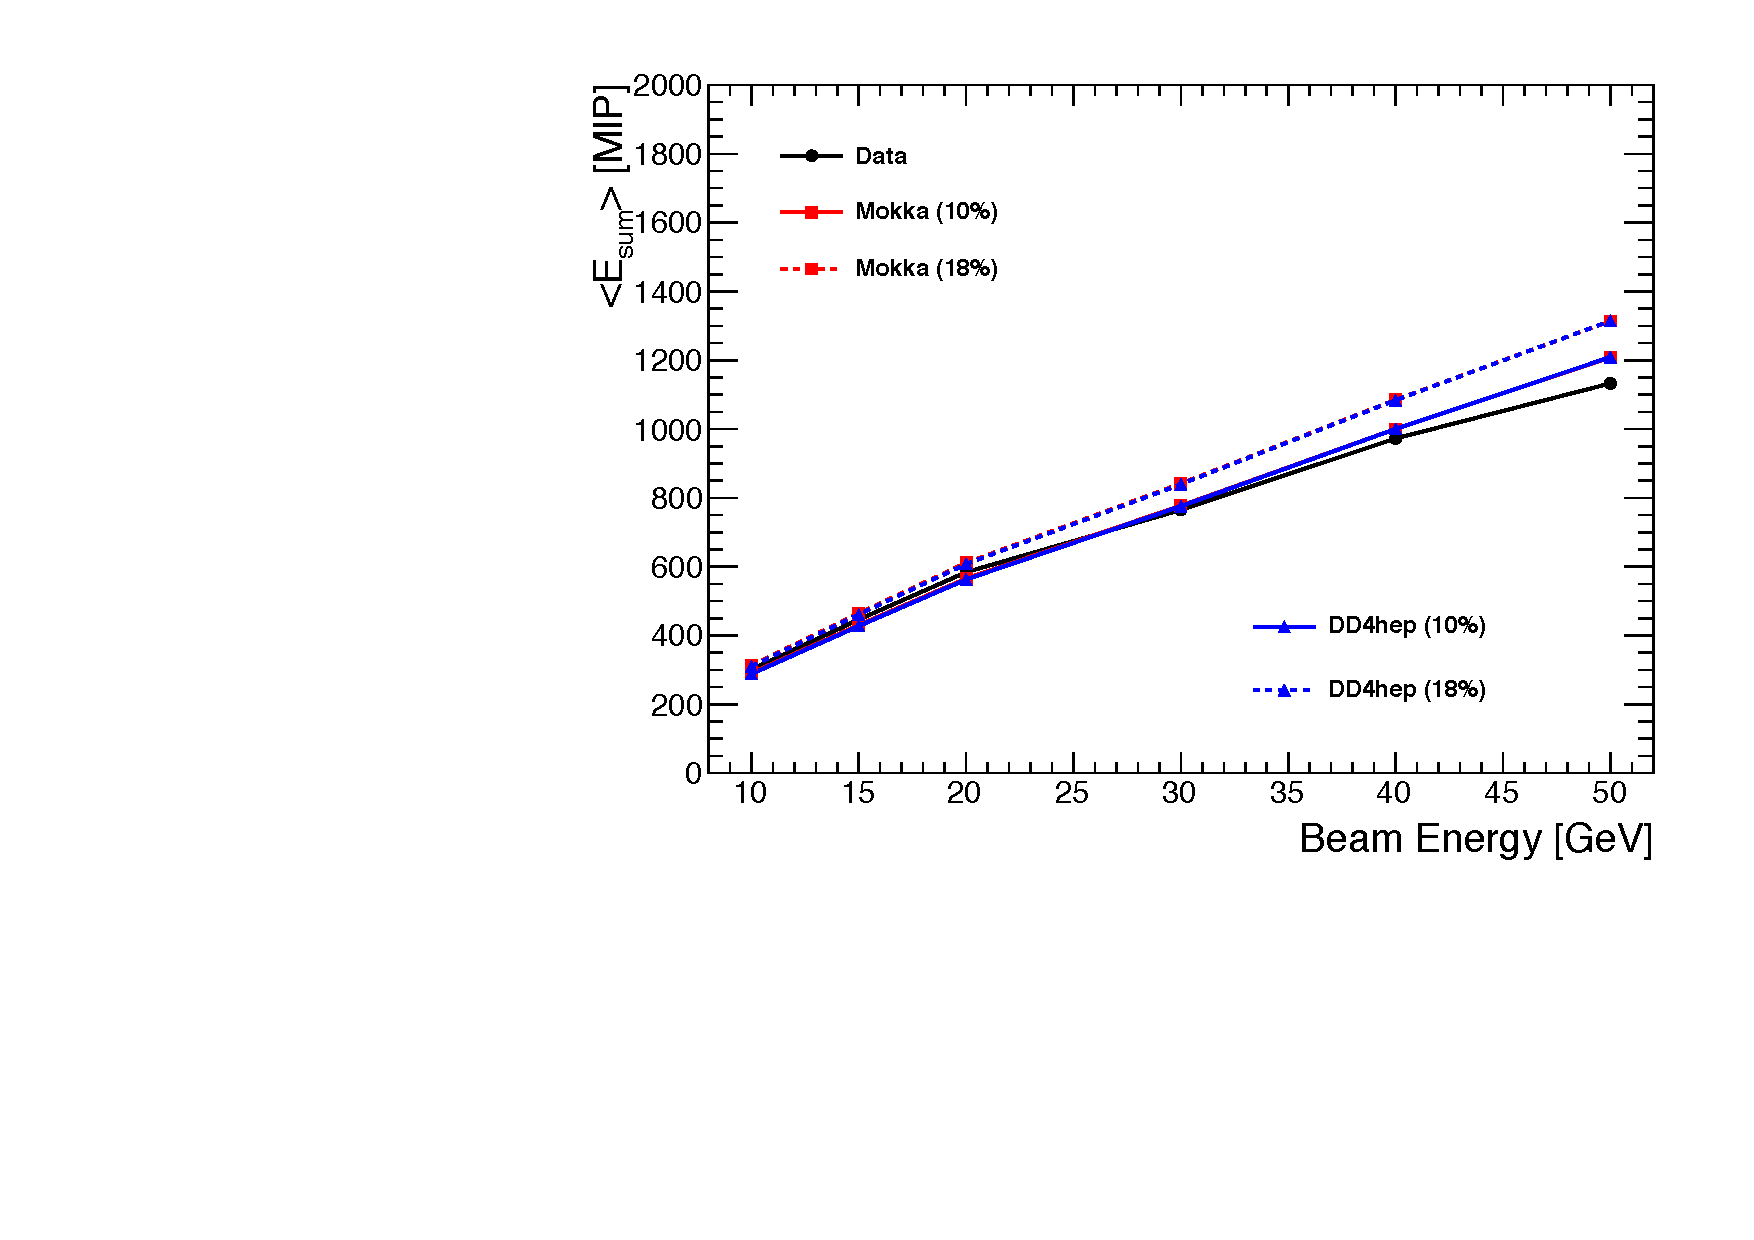
\includegraphics[width=1.\linewidth]{chap5/fig_AHCAL_Timing/Electrons/EsumElectrons_BeamEnergy.pdf}
    \caption{} \label{fig:EsumMean}
  \end{subfigure}
  \hfill
  \begin{subfigure}[t]{0.49\textwidth}
    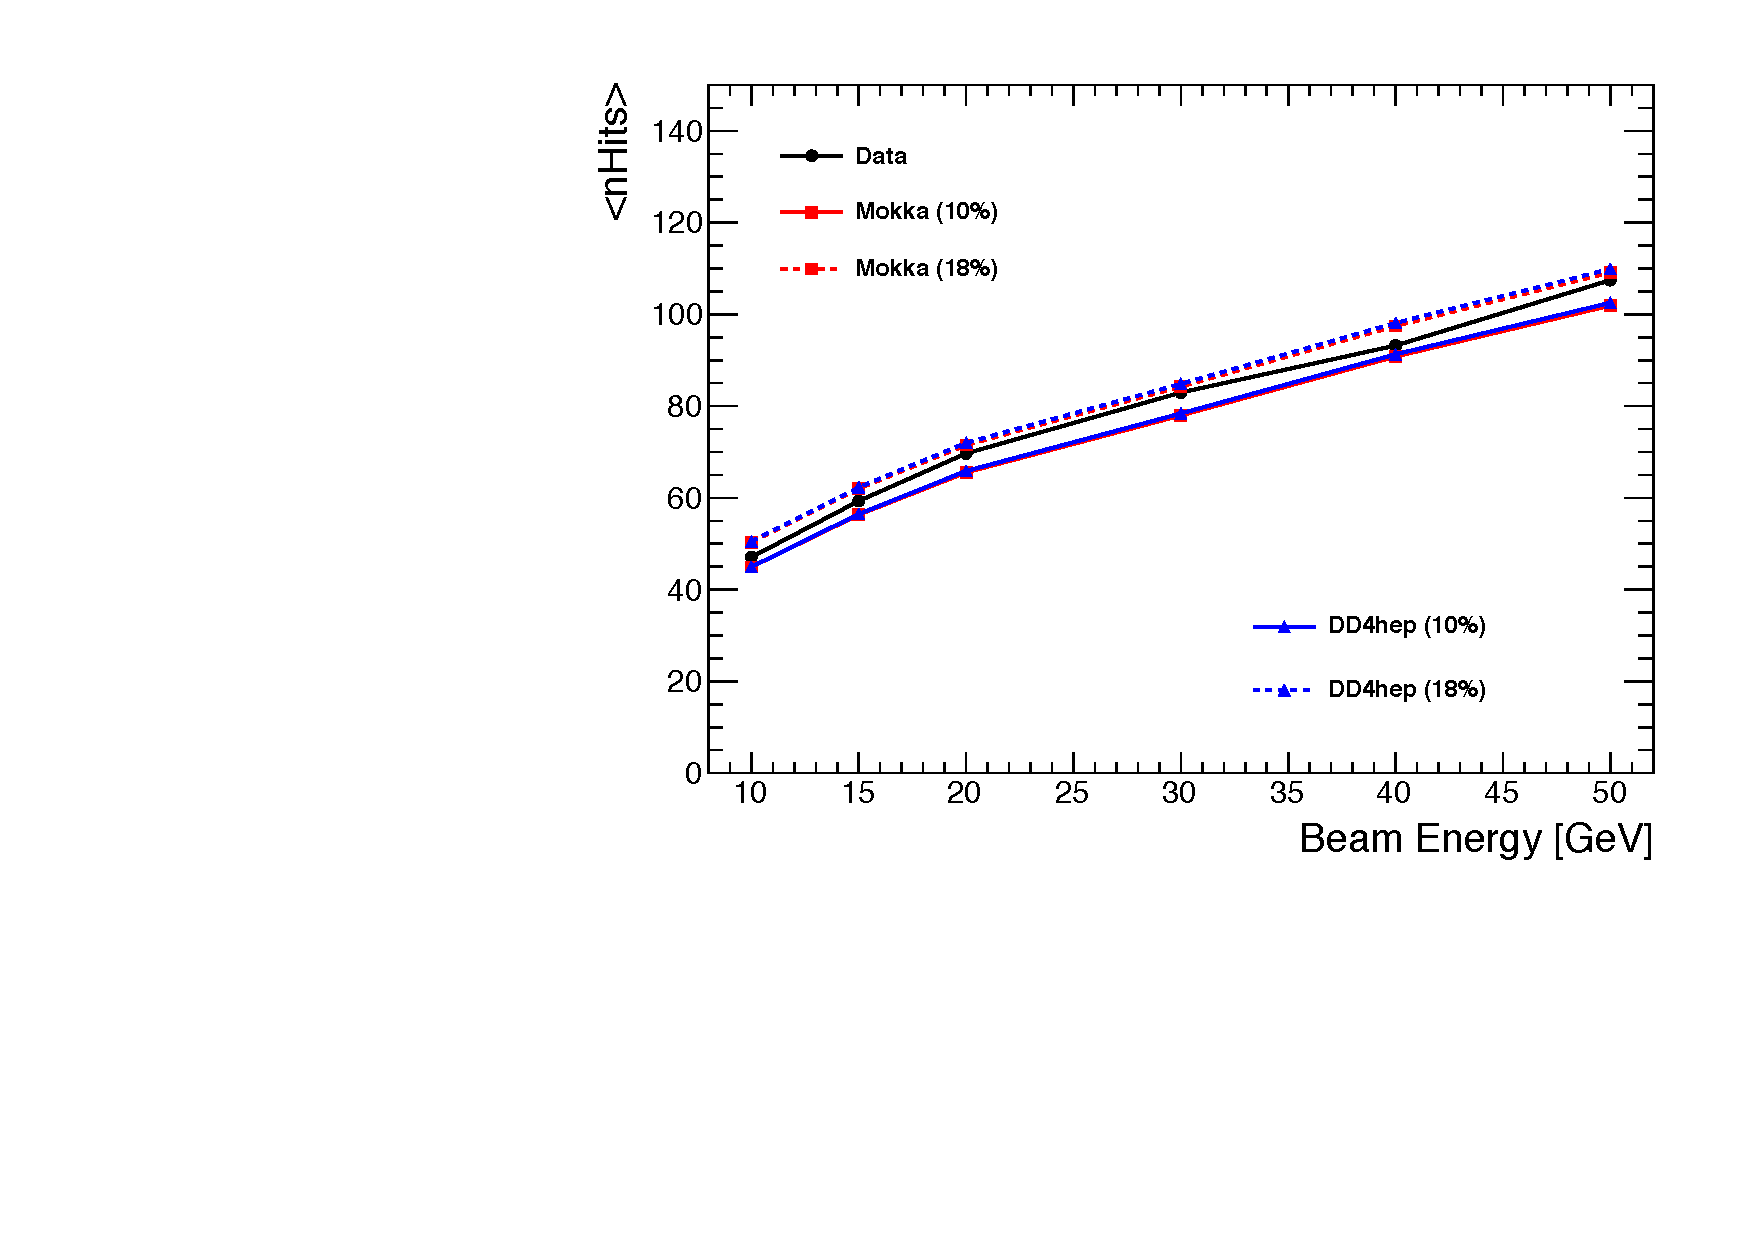
\includegraphics[width=1.\linewidth]{chap5/fig_AHCAL_Timing/Electrons/nHitsElectrons_BeamEnergy.pdf}
    \caption{} \label{fig:nHitsMean}
  \end{subfigure}
  \caption{\subref{fig:EsumMean}) Comparison of the mean energy sum in the AHCAL as function of the beam energy for electron data and simulations with different cross-talk parameters. \subref{fig:nHitsMean}) Comparison of the mean number of hits in the AHCAL as function of the beam energy for electron data and simulations with different cross-talk parameters.}
  \label{fig:eVal}
\end{figure}

The investigation of these observables enables us to validate the simulations to a certain degree of confidence between 5-20\% with the data. The precision of the detector simulation for electrons is limited by the cross-talk simulation and for energies above 20 GeV, by the possible contamination by low energy electrons in the data. A deeper investigation on the energy aspect of the data is carried out in parallel of this analysis \cite{AmbraEnergy}.
